\documentclass[aspectratio=169,11pt]{beamer}
\usepackage{teaching_slides}


\title{Instrumental Variables}
\author{Chris Conlon}
\institute{Applied Econometrics}
\date{\today}

%\usepackage[italic]{mathastext}



%\usepackage{caption,subcaption}
%\usepackage{booktabs}
%\usepackage[flushleft]{threeparttable}


% \usepackage{tikz}
% \usepackage{pgfplots}
% \pgfplotsset{compat=1.7}
% \usetikzlibrary{arrows, shapes, snakes, patterns, angles, quotes}




\begin{document}

\maketitle

\begin{frame}{Basic Idea}
\begin{itemize}
	\item Basic Idea of Instrumental Variable (IV):
		\begin{itemize}
			\item What if we have a variable that is correlated with $X$ \emph{but not with $Y$}
			\item Then any changes in $Y$ caused by that variable will reflect causal changes by $X$
		\end{itemize}
\medskip
\item Equation of interest:
\begin{align*}
	Y_i = \beta_0 + \beta_1 X_i + \varepsilon_i
\end{align*}
	\item IVs break $X$ into two pieces that are themselves uncorrelated:
		\begin{align*}
			X_i =\gamma_0 + \gamma_1  Z_i + \eta_i
		\end{align*}

		\begin{itemize}
			\item A piece that is not correlated with $\varepsilon$ ($Cov(Z,\varepsilon)=0$)
			\item A piece that is correlated with $\varepsilon$ ($Cov(\eta,\varepsilon)\ne0$) -- source of the endogeneity problem
			\item Finally, $Cov(Z,\eta)=0$
		\end{itemize}
	\item $Z_i$ is an {\bf instrumental variable}
\end{itemize}
\end{frame}



\begin{frame}{Terminology Review}

A ``Good" Regression:

% \begin{figure}[H]
% \begin{center}
% \resizebox{.4\textwidth}{!}{
% \begin{tikzpicture}

% \tikzset{vertex/.style = {shape=circle,draw,minimum size=1em}}
% \tikzset{edge1/.style = {->,thick,> = latex',shorten <=2pt}}
% \tikzset{edge2/.style = {<-,thick, > = latex', shorten <=3pt, dashed}}
% % vertices
% \node[vertex] (a) at  (0,0) {\makebox[7.5mm][c]{\small X}};;
% \node[vertex] (b) at  (5,0) {\makebox[7.5mm][c]{\small  $\varepsilon$}};;
% \node[vertex] (c) at  (2.5,-2) {\makebox[7.5mm][c]{\small Y}};
% %\node (d) at (2.5,0) {??};
% \node at (2.5,.66) {Exogenous};
% \node at (2.5,-2.75) {Endogenous};

% %edges
% \draw[edge1] (a) to (c);
% \draw[edge1] (b) to (c);
% %\draw[edge2] (a) to (d);
% %\draw[edge2] (b) to (d);                                            v

% % rectangle
% \draw[rounded corners=15pt]
%   (-1,-.75) rectangle ++(7,1.65);

% \draw[rounded corners=15pt]
%   (-1,-3.25) rectangle ++(7,2);

% \end{tikzpicture}}
% \end{center}
% \end{figure}

\begin{itemize}{\small
	\item {\bf Exogenous Variables:} Variables in the data that do not cause each other
		\begin{itemize}
			\item $\varepsilon$ is always exogenous, so exogenous also just means variables not correlated with $\varepsilon$
		\end{itemize}
	\item {\bf Endogenous Variables:} Variables that are determined by exogenous variables in the model
		\begin{itemize}
			\item $\varepsilon$ is always in $Y$ so $Y$ is always endogenous
		\end{itemize}}
\end{itemize}
\end{frame}


\begin{frame}{Omitted Variable Bias with Pictures}

Selection/OVB:

% \begin{figure}[H]
% \begin{center}
% \resizebox{.4\textwidth}{!}{
% \begin{tikzpicture}

% \tikzset{vertex/.style = {shape=circle,draw,minimum size=1em}}
% \tikzset{edge1/.style = {->,thick,> = latex',shorten <=2pt}}
% \tikzset{edge2/.style = {<-,thick, > = latex', shorten <=3pt, dashed}}
% % vertices
% \node[vertex] (a) at  (0,-2) {\makebox[6mm][c]{\small X}};;
% \node[vertex] (b) at  (2.5,-.1) {\makebox[6mm][c]{\small  $\varepsilon$}};;
% \node[vertex] (c) at  (5,-2) {\makebox[6mm][c]{\small Y}};
% %\node (d) at (2.5,0) {??};
% \node at (2.5,.66) {Exogenous};
% \node at (2.5,-2.75) {Endogenous};

% %edges
% \draw[edge1] (a) to (c);
% \draw[edge1] (b) to (c);
% \draw[edge2] (a) to (b);
% %\draw[edge2] (b) to (d);                                            v

% % rectangle
% \draw[rounded corners=15pt]
%   (-1,-.75) rectangle ++(7,1.65);

% \draw[rounded corners=15pt]
%   (-1,-3.25) rectangle ++(7,2);

% \end{tikzpicture}}
% \end{center}
% \end{figure}

\begin{itemize}{\small
	\item In this picture $X$ is {\bf endogenous} because $\varepsilon$ now causes $X$ as well
	\item What if there is another exogenous variable that \emph{does not} directly cause $Y$?
	}
\end{itemize}


\end{frame}


\begin{frame}{Omitted Variable Bias with Pictures}

Instrumental Variable:

% \begin{figure}[H]
% \begin{center}
% \resizebox{.4\textwidth}{!}{
% \begin{tikzpicture}

% \tikzset{vertex/.style = {shape=circle,draw,minimum size=1em}}
% \tikzset{edge1/.style = {->,thick,> = latex',shorten <=2pt}}
% \tikzset{edge2/.style = {<-,thick, > = latex', shorten <=3pt, dashed}}
% % vertices
% \node[vertex] (a) at  (0,-2) {\makebox[6mm][c]{\small X}};;
% \node[vertex] (b) at  (4,-.1) {\makebox[6mm][c]{\small  $\varepsilon$}};;
% \node[vertex] (c) at  (5,-2) {\makebox[6mm][c]{\small Y}};
% \node[vertex] (d) at  (1,-.1) {\makebox[6mm][c]{\small  Z}};;
% %\node (d) at (2.5,0) {??};
% \node at (2.5,.66) {Exogenous};
% \node at (2.5,-2.75) {Endogenous};

% %edges
% \draw[edge1] (a) to (c);
% \draw[edge1] (b) to (c);
% \draw[edge2] (a) to (b);
% \draw[edge1] (d) to (a);                                            v

% % rectangle
% \draw[rounded corners=15pt]
%   (-1,-.75) rectangle ++(7,1.65);

% \draw[rounded corners=15pt]
%   (-1,-3.25) rectangle ++(7,2);

% \end{tikzpicture}}
% \end{center}
% \end{figure}

\begin{itemize}{\small
	\item $Z$ causes $Y$ \emph{only indirectly} through $X$
	\item We can estimate ``causal effect" of $Z$ on $Y$ and this MUST be the causal effect of $Z$ on $X$ and the causal effect of $X$ on $Y$
	\begin{itemize}
		\item Mathematically we need to split effect of on $Z$ on $Y$ into effect of $Z$ on $X$ and $X$ on $Y$
		\item Related concept in statistics: Path Analysis
	\end{itemize}
	}
\end{itemize}
\end{frame}

\begin{frame}{Formal Definition of an Instrumental Variable}
Model:
\begin{align*}
	Y_i = \beta_0 + \beta_1 X_i + \varepsilon_i
\end{align*}

\begin{itemize}
\item We call a variable $Z$ a a valid {\bf instrumental variable} if the following two conditions hold:
\end{itemize}
\begin{enumerate}
	\item {\bf Relevance:} $Cov(X,Z)\ne 0$
		\begin{itemize}
			\item An arrow from $Z$ to $X$ in the pictures
		\end{itemize}
\medskip
	\item {\bf Exogeneity:} $Cov(\varepsilon,Z)= 0$
		\begin{itemize}
			\item No arrow from $Z$ to $Y$ or $Z$ to $\varepsilon$ in the picture
		\end{itemize}
\end{enumerate}
\end{frame}

\begin{frame}{Key Assumption \#1 of Instrumental Variables}
\begin{itemize}
	\item {\bf Relevance:} $Cov(X,Z)\ne 0$
\medskip
\item This assumption just means that $X$ and $Z$ are correlated
\medskip
\item We observe both $X$ and $Z$, so can easily test this assumption by regressing:
\begin{align*}
X_i = \beta_0 + \beta_1 Z_i + \varepsilon_i
\end{align*}
\item If $\beta_1 \neq 0$ in regression, we say instrument is relevant
\end{itemize}
\end{frame}

\begin{frame}{Key Assumptions \#2 of Instrumental Variables}
\begin{itemize}
	\item {\bf Exogeneity (or validity):} $Cov(\varepsilon,Z)= 0$
\medskip
\item This assumption means that $Z$ and $\varepsilon$ cannot be correlated
\medskip
\item We do not observe $\varepsilon$, so we \textbf{cannot} test this assumption
\medskip
\item In general, we need to ``defend" this assumption by telling a story about why $Z$ and $\varepsilon$ are unlikely to be correlated
\medskip
\item Much like parallel trends or strict exogeneity, these crucial identifying assumptions cannot
be tested on their own. However, we can test them against each other. That is, the best we can
do is ask the question "given this exogeneity assumption, does this other exogeneity assumption seem
true?" But we can never test an exogeneity assumption in a self-contained way. 
\end{itemize}
\end{frame}

\begin{frame}{Best Defense of Exogeneity IV Assumption: Randomized Experiment}
\begin{itemize}
\item Back to the class size example:
\begin{align*}
score_i = \beta_0 + \beta_1 \textit{CS}_i + \varepsilon_i
\end{align*}
\item where:
\begin{itemize}
\item $score_i$: Test score of student $i$
\item $CS_i$: Class size of student $i$
\end{itemize}
\medskip
\item Suppose that we use a coin flip that sends kids that get a ``head" to a small class and kids getting a ``tails" to big class
\begin{itemize}
\item This is our randomized experiment!
\end{itemize}
\medskip
\item Let's call the coin flip our instrument $Z$ (where $Z_i=1$ if heads, $Z_i=0$ if tails)
\end{itemize}
\end{frame}

\begin{frame}{Best Defense of Exogeneity IV Assumption: Randomized Experiment}
\vspace{-0.5em}
\begin{align*}
score_i = \beta_0 + \beta_1 \textit{CS}_i + \varepsilon_i
\end{align*}
\begin{itemize}
\item Is $Z$ (our coin flip) a good instrument?
\medskip
\item {\bf Relevance:} $Cov(CS,Z)\ne 0$? Yes, if $Z_i=1$ kid gets small class, if $Z_i=0$ kid gets big class
\begin{itemize}
\item So the regression $CS_i=\beta_0 + \beta_1 Z_i + \varepsilon_i$ will estimate that $\beta_1<0$
\end{itemize}
\medskip
\item {\bf Exogeneity:} $Cov(\varepsilon,Z)\ne 0$? Untestable -- so need to tell a story
\begin{itemize}
\item Story: Exogeneity holds because coin flip is random and does not depend on any student or parent characteristics that would affect test scores.  Therefore, there is nothing related to $Z$ (besides $X$) that is also related to test scores, so $\varepsilon$ and $Z$ must be uncorrelated.\\
This is a good story! It's the ``magic'' of randomization.
\end{itemize}
\end{itemize}
\end{frame}

\begin{frame}{ Randomized Experiment as an IV}
\begin{itemize}
\item So a randomized experiment can be treated as an IV, but there is a big difference in
	how we evaluate the assumption for an experimental or non-experimental setting
\medskip
\item When running an experiment, the exogeneity assumption is justified if the
	randomization was implemented in way that was not correlated with anything else that could
	influence outcomes. Attrition and manipulation can undermine exogeneity in an experimental context
	if they create a correlation between treatment status and other factors that might influence outcomes.
	 Thus, exogeneity amounts to an assumption about how the randomization was implemented.
	\medskip
	\item In contrast, the IV exogeneity assumption in a non-experimental context is a broad and vague statement
	about how the world works; it's much more difficult to interpret and evaluate. The same is
	true of strict exogeneity or parallel trends.
\end{itemize}
\end{frame}


\begin{frame}{IV Estimation: Example with a 0/1 $Z$}

Let's begin with the simplest 0/1 model (this time for $Z$):
\begin{align*}
	Y_i = \beta_0 + \beta_1 X_i + \varepsilon_i\\
\end{align*}

\begin{itemize}
	\item  $X$ is endogenous but we have a 0/1 instrument, $Z$
	\begin{itemize}
		\item Because $Z$ is 0/1 we can focus on group means.
	\end{itemize}

	\item What assumptions do we need to make?
		\begin{itemize}
			\item $Cov(X,Z)\ne 0$
			\item $Cov(Z,\varepsilon) = 0$
		\end{itemize}
	\item The intuition from above: solve for the ``indirect" effect of $Z$ on $Y$
\end{itemize}

\end{frame}





\begin{frame}{The Relationship Between $Y$ on $Z$}

What is the relationship between $Y$ and $Z$, taking expectations?
\begin{align*}
		\E(Y|Z) =& E\left(\beta_0 + \beta_1 X + \varepsilon| Z\right)\\
			   =& \beta_0 + \beta_1 \E(X|Z) + \underbrace{\E(\varepsilon|Z)}_{=0}\\
			   =&\beta_0 + \beta_1 \E(X|Z)
\end{align*}

Since $Z$ is 0/1... 

\begin{align*}
	\E(Y|Z=1) =& \beta_0 + \beta_1 \E(X|Z=1)\\
	\E(Y|Z=0) =& \beta_0 + \beta_1 \E(X|Z=0)
\end{align*}

Rearranging... 
\begin{align*}
	\E(Y|Z=1)-\E(Y|Z=0) = \beta_1\times\left(\E(X|Z=1)-\E(X|Z=0)\right)
\end{align*}



\end{frame}

\begin{frame}{The IV Regression for a 0/1 $Z$}

From the previous slide we have:
\begin{align*}
	\beta_1 = \frac{E(Y|Z=1)-E(Y|Z=0)}{E(X|Z=1)-E(X|Z=0)}
\end{align*}


From the LLN we can construct the following estimator:
		\begin{align*}
			\hat\beta_1 = \frac{\bar Y_1 - \bar Y_0}{\bar X_1 - \bar X_0}
		\end{align*}
		\begin{itemize}
			\item The subscript refers to $Z=1$ or $Z=0$
			\item We call this the IV estimator
		\end{itemize}


\end{frame}

\begin{frame}{Interpreting the Estimator for 0/1 $Z$}

Estimator:
	\begin{align*}
			\hat\beta_1^{IV} = \frac{\bar Y_1 - \bar Y_0}{\bar X_1 - \bar X_0}
	\end{align*}

\begin{itemize}

	\item For a 0/1 $X$ we look at the change in $Y$ over the change in $X$:
		\begin{align*}
			\hat\beta_1^{OLS} = \frac{\bar Y_{X=1} - \bar Y_{X=0}}{\bar X_{X=1} - \bar X_{X=0}} = \Delta \bar Y
		\end{align*}

	\begin{itemize}
		\item For a $0/1$ $X$, $\Delta \bar X = 1$
		\item Basically looking at how much $Y$ changes for a change in $X$
	\end{itemize}

	\item Intuition for a 0/1 $Z$
		\begin{itemize}
			\item The effect of $X$ on $Y$ is still the change in $Y$ over a change in $X$
			\item Use the change in $Y$ \emph{given $Z$} to shut down the effects of $\varepsilon$
			\item Use the change in $X$ \emph{given $Z$} to get the right scaling
		\end{itemize}
\end{itemize}
\end{frame}


\begin{frame}{The IV  Regression with a Continuous $Z$}

Same model as before:
\begin{align*}
	Y_i = \beta_0 + \beta_1 X_i + \varepsilon_i
\end{align*}



\begin{itemize}
	\item Now assume that $Z$ is continuous
	\item How to capture the indirect effect of $Z$?
		\begin{itemize}
			\item Intuition from OLS: use the covariance between $Z$ and $Y$ as a measure of the relationship:
	\begin{align*}
	Cov(Y,Z) =& Cov(\beta_0 + \beta_1 X + \varepsilon,Z)\\
			 =& \beta_1 Cov(X,Z)
	\end{align*}
			\item Rearranging:
				\begin{align*}
					\beta_1= \frac{Cov(Y,Z)}{Cov(X,Z)}
				\end{align*}
		\end{itemize}
	\item {\bf Instrumental Variables Estimator:}
		\begin{align*}
			\hat\beta^{IV}_1 = \frac{s_{YZ}}{s_{XZ}}
		\end{align*}
\end{itemize}
\end{frame}







\begin{frame}{Heterogeneous treatment effects I}
\begin{itemize}
\item Let's consider a simple case with binary treatment $X_i \in \left\{0,1\right\}$ where 
the treatment effect $\beta_i=\E\left(Y_{i1} - Y_{i0}\right)$ is heterogeneous.
\begin{itemize}
	\item $Y_{ix}$ denotes the potential outcome for $i$ given treatment status $X_i = x$.
\end{itemize}

\medskip
\item We have a binary instrument $Z_i \in \left\{0,1\right\}$

\medskip
\item Let's also have potential outcomes for treatment status: $X_{iz}$ is the potential
	treatment status for $i$ when $Z_i = z$. 

\medskip
\item Model:
\begin{align*}
	Y_i = \beta_0 + \beta_i X_i + \varepsilon_i
\end{align*}


\end{itemize}
\end{frame}

\begin{frame}{Heterogeneous treatment effects II}
\begin{align*}
	Y_i = \beta_0 + \beta_i X_i + \varepsilon_i
\end{align*}

\begin{itemize}
\item Assuming that $\E\left[\varepsilon_i | Z_i = 1\right] - \E\left[\varepsilon_i | Z_i = 0\right] =0$,
\begin{align*}
\E\left[ Y_i | Z_i = 1\right] - \E\left[ Y_i | Z_i = 0\right] = \E\left[ \beta_i X_i | Z_i = 1\right] - \E\left[ \beta_i X_i | Z_i = 0\right] 
\end{align*}

\medskip
Plugging in our potential outcomes for $X$,
\begin{align*}
\E\left[ Y_i | Z_i = 1\right] - \E\left[ Y_i | Z_i = 0\right] = \E\left[ \beta_i \left(X_{i1} -X_{i0}\right) \right] 
\end{align*}

\end{itemize}
\end{frame}

\begin{frame}{Heterogeneous treatment effects III}
\begin{align*}
\E\left[ Y_i | Z_i = 1\right] - \E\left[ Y_i | Z_i = 0\right] = \E\left[ \beta_i \left(X_{i1} -X_{i0}\right) \right] 
\end{align*}

\begin{itemize}
\item Given the binary treatment, there are three possible values for $X_{i1} -X_{i0}$:
\begin{align*}
\footnotesize
\begin{array}{llcl}
\E\left[\beta_{i}\left(X_{i1}-X_{i0}\right)\right] & =\Pr\left(X_{i1}-X_{i0}=1\right)\E\left[\beta_{i}\left(X_{i1}-X_{i0}\right)|X_{i1}-X_{i0}=1\right] & \qquad & \text{(compliers)}\\
 & +\Pr\left(X_{i1}-X_{i0}=0\right)\E\left[\beta_{i}\left(X_{i1}-X_{i0}\right)|X_{i1}-X_{i0}=0\right] &  & \text{(always/never takers)}\\
 & +\Pr\left(X_{i1}-X_{i0}=-1\right)\E\left[\beta_{i}\left(X_{i1}-X_{i0}\right)|X_{i1}-X_{i0}=-1\right] &  & \text{(defiers)}
\end{array}
\end{align*}


\item The second term (always/never takers) is necessarily equal to zero. We might also make a {\bf monotonicity assumption} that
	$\Pr\left(X_{i1}-X_{i0}=-1\right)=0$. Ruling out defiers, this could be interpreted to mean that 
	being assigned to treatment can only make you more likely to receive treatment.
	
\end{itemize}
\end{frame}



\begin{frame}{Heterogeneous treatment effects IV}
\[
E\left[ Y_i | Z_i = 1\right] - E\left[ Y_i | Z_i = 0\right] = E\left[ \beta_i \left(X_{i1} -X_{i0}\right) \right] 
\]
\begin{itemize}
\item With monotonicity, we have \[
E\left[\beta_{i}\left(X_{i1}-X_{i0}\right)\right]  = Pr\left(X_{i1}-X_{i0}=1\right)E\left[\beta_{i}\left(X_{i1}-X_{i0}\right)|X_{i1}-X_{i0}=1\right]
\]

\item Also note that $Pr\left(X_{i1}-X_{i0}=1\right) = E\left[ X_{i} | Z_i=1\right] - E\left[ X_{i} | Z_i=0\right]$

\item Combining the above,\[
\frac{E\left[ Y_i | Z_i = 1\right] - E\left[ Y_i | Z_i = 0\right] }{E\left[ X_{i} | Z_i=1\right] - E\left[ X_{i} | Z_i=0\right]} = E\left[\beta_{i}\left(X_{i1}-X_{i0}\right)|X_{i1}-X_{i0}=1\right]
= E\left[\beta_{i}|X_{i1}-X_{i0}=1\right]
\]

\item We now have that our IV estimator equals the {\bf local average treatment effect}, which means the average effect on the individuals whose treatment
status is changed by the instrument. 

\end{itemize}
\end{frame}





\begin{frame}{IV Example}
\begin{itemize}

\item Suppose that we are interested in investigating the effect of studying on grades:
\begin{align*}
Y_i=\beta_0 + \beta_1 X_i + \varepsilon_i
\end{align*}
\item where
\begin{itemize}
\item $Y_i$: is GPA
\item $X_i$: is study time (hours per day)
\end{itemize}
\medskip
\item We expect that our OLS estimator $\hat{\beta}_1$ will be severely biased here (why?)
\end{itemize}
\end{frame}

\begin{frame}{IV Model}
\begin{itemize}
\item To get rid of OVB, we shall use an IV
\medskip
\item One possible IV: whether your roommate has a N64 (or playstation/whatever video game console kids use today)
\medskip
\item Important feature: Roommates are randomly assigned in college
\begin{itemize}
\item At least at Berea College (Kentucky) where this example comes from (see Stinebrickner and Stinebrickner (2008))
\end{itemize}
\end{itemize}
\end{frame}

\begin{frame}{Instrument Validity}
\begin{itemize}
\item First thing for any instrument is to think of validity. Two conditions:
\begin{itemize}
\item Instrument is $N64$, which is indicator variable that your roommate has N64
\end{itemize}
\end{itemize}
\begin{enumerate}
\item Relevance: $Cov(Z,X)\neq 0$; here $Cov(N64,study)\neq 0$
\begin{itemize}
\item Seems likely to hold as everyone prefers playing Mario Kart to studying
\item Testable
\end{itemize}
\medskip
\item Exogeneity: $Cov(Z,\varepsilon)= 0$; here $Cov(N64,\varepsilon)=0$
\begin{itemize}
\item Untestable
\item Is it plausible? 
\end{itemize}
\end{enumerate}
\end{frame}

\begin{frame}{Thinking About Exogeneity}
\begin{itemize}
\item Exogeneity: $Cov(Z,\varepsilon)= 0$
\medskip
\item ``Storytime" should talk about how two things hold
\begin{enumerate}
\item People select into $Z$ in some manner that is likely to be correlated with $Y$
\begin{itemize}
\item Concern: People that pick roommates that are ``fun" and have N64s are likely people who do not care too much about grades
\end{itemize}
\item $Z$ only affects $Y$ through $X$
\begin{itemize}
\item Concern: Having a roommate with a video game affects your GPA through other means than affecting your study hours
\end{itemize}
\end{enumerate}
\medskip
\item Either story ``invalidates" the instrument (but in different ways)
\end{itemize}
\end{frame}

\begin{frame}{Thinking About Exogeneity}
\begin{enumerate}
\item Selection story: there is an omitted variable related to both $Z$ and $Y$
\begin{itemize}
\item Example: omitted variable is effort because students that really put in a lot of effort make sure they do not get a roommate with N64
\end{itemize}
\medskip
\item Other channel story:
\begin{itemize}
\item Possible Story 1: Mario Kart helps me grasp physics, so I ace my physics exam
\begin{itemize}
\item so $Z$ directly affects Y \emph{independent} of $X$
\end{itemize}
\item Possible Story 2: Other people hang out in our room due to our N64, making it really loud and so I cannot study effectively
\begin{itemize}
\item so $Z$ affects Y through \emph{another} $X$
\end{itemize}



\end{itemize}
\end{enumerate}
\begin{itemize}
\item Conceptually, there are two aspects to the exogeneity assumption: {\bf randomization} and {\bf exclusion}.
Be careful: even when an IV is clearly random, it might not be excludable. 
\end{itemize}
\end{frame}

\section{IV Math}
\begin{frame}{IV Directly into Model}
\begin{itemize}
\item Suppose that our IV assumptions hold
\medskip
\item Then we can just directly replace $X$ with our IV in our model:
\begin{align*}
Y_i=\pi_0 + \pi_1 Z_i + \varepsilon_i
\end{align*}
\item where
\begin{itemize}
\item $Y_i$: is GPA
\item $Z_i$: is whether roommate has N64
\end{itemize}
\medskip
\item \textbf{Interpretation of $\hat{\beta}_1$:} Having a roommate with a N64 \textbf{causes} a $\hat{\beta}_1$ decrease in GPA
\begin{itemize}
\item Causal effect because validity of instrument, $cov(Z,\varepsilon)=0$, implies OLS is consistent for above equation.
Of course we could question the instrument's validity.
\end{itemize}
\medskip
\item But we want the effect of \emph{studying} on GPA!
\end{itemize}
\end{frame}

\begin{frame}{Two Stage Least Squares}
\begin{itemize}
\item A popular IV estimator is Two Stage Least Squares (2SLS)
\medskip
\item This effectively runs regression $Y_i=\beta_0 + \beta_1 Z_i + \varepsilon_i$, but \emph{scales} $\beta_1$ by how much $Z$ affects $X$
\begin{itemize}
\item If $Z$ affects $X$ at one-to-one rate, $\beta_1$ in above regression will capture effect of $X$
\item If $Z$ affects $X$ only a little, we need to scale $\beta_1$ up a lot to say what effect of $X$ on $Y$ is
\end{itemize}
\medskip
\item We therefore estimate in two steps:
\begin{enumerate}
\item Regress $X$ on $Z$ to capture effect of $Z$ on $X$
\item Regress fitted values of step 1 to capture effect of $X$ on $Y$
\end{enumerate}
\smallskip
\item Under IV assumptions, this gives us \textbf{causal} effect of $X$ on $Y$
\end{itemize}
\end{frame}

\begin{frame}{2SLS Implementation}
\begin{itemize}
\item Step 1: regress
\begin{align*}
X_i=\pi_0 + \pi_1 Z_i + \eta_i
\end{align*}
\item Step 2: take your predicted values from Step 1, $\hat{X}_i$, and regress
\begin{align*}
Y_i=\gamma_0 + \gamma_1 \hat{X}_i + \varepsilon_i
\end{align*}
\item Under IV assumptions, step 1 finds the ``good part" of $X$ (that is not related to $\varepsilon$), and then step 2 takes that ``good part" of $X$ as a regression to find the causal relationship between $X$ and $Y$
\end{itemize}
\end{frame}


%\begin{frame}{2SLS Estimator}
%\begin{itemize}
%\item Why is $\hat{\beta}_1^{2SLS}=\frac{Cov(Y,Z)}{Cov(X,Z)}$?
%\medskip
%\item True model:
%\begin{align*}
%Y_i=\beta_0 + \beta_1 X_i + \varepsilon_i
%\end{align*}
%\item Take covariance of both sides with respect to $Z$:
%\begin{align*}
%Cov(Y_i, Z_i)&=Cov(\beta_0 + \beta_1 X_i + \varepsilon_i, Z_i) \\
%Cov(Y_i, Z_i)& = Cov(\beta_0, Z_i) + Cov(\beta_1 X_i, Z_i) + Cov(\varepsilon_i, Z_i)\\
%Cov(Y_i, Z_i)& = 0 + \beta_1Cov( X_i, Z_i) +0 \;\; \textit{since $Cov(\varepsilon_i, Z_i)$ by assumption} \\
%\implies & \beta_1 =\frac{Cov(Y,Z)}{Cov(X,Z)}
%\end{align*}
%\end{itemize}
%\end{frame}


\begin{frame}[fragile]\frametitle{Single Variable IV in \texttt{R}: Manually}
\begin{itemize}
\item Data:
\begin{itemize}
\item $Y_i$: is GPA
\item $X_i$: is study time (hours per day)
\item $Z_i$: is indicator for roomate having N64
\end{itemize}
\medskip
\item Running 2SLS by doing both steps manually:
\medskip
\item Step 1: Regress $X_i=\pi_0 + \pi_1 Z_i + v_i$ and get predicted study time, $\hat{X}_i$
\begin{itemize}
\item Data\$xHat = predict(lm(X$\sim$Z, data=Data))
\end{itemize}
\item Step 2: Regress $y_i=\gamma_0 + \gamma_1 \hat{X}_i + \varepsilon_i$
\begin{itemize}
\item m3 = lm(Y$\sim$xHat, data=Data)
\item coeftest(m3, vcov = vcovHC(m3, type = ``HC1"))
\begin{itemize}
\item Note: Standard errors will be wrong!
\end{itemize}
\end{itemize}
	\begin{itemize}{\small
		\item \texttt{predict} gives the fitted values of $X$ from the first stage
		\item Then \texttt{lm} can be used to get the second stage
		\item Problem: the standard errors (even robust) will be wrong}
	\end{itemize}
	\end{itemize}
\end{frame}

\begin{frame}[fragile]\frametitle{Doing Single Variable IV in \texttt{R}: All at once}
\begin{itemize}
\item Need a package called \texttt{AER} for this
\begin{itemize}
\item install.packages(``AER")
\item library(AER)
\end{itemize}
\medskip
\item \texttt{R} can run 2SLS all at once:
\medskip
\item m4 = ivreg(Y $\sim$ X $|$ Z, data=Data)
\medskip
\item Use new standard error command to get ``right" standard errors:
\begin{itemize}
\item coeftest(m4, vcov=sandwich)
\end{itemize}
	\end{itemize}
\end{frame}



\begin{frame}{IV Setup with Matrix Notation}
\begin{itemize}
\item Consider a multiple regression equation
\begin{align*}
\boldsymbol{y}=\boldsymbol{\beta}\boldsymbol{X}+\boldsymbol{\varepsilon}
\end{align*}
The IV assumptions are now that
\begin{itemize}
\item $Cov\left(\boldsymbol{z}_{i},\varepsilon_{i}\right)=\boldsymbol{0}$
\item $Cov\left(\boldsymbol{z}_{i},\boldsymbol{x}_{i}\right)$ has \emph{full rank}, i.e., rank $K$, where $K$ is
	the number of regressors in $\bf{x}$
\end{itemize}
\item We can have multiple regressors as well as instruments. Some regressors can also be instruments; if $\boldsymbol{z}_{i}=\boldsymbol{x}_{i}$
then we can just use OLS.
\item Regressors that are instruments are \textbf{exogenous regressors}.
Regressors that are not instruments are \textbf{endogenous regressors}.
\item For the rank assumption, we need at least one instrument for each
endogenous regressor.
\end{itemize}
\end{frame}


\begin{frame}{2SLS with Matrix Notation}
\begin{itemize}
\item The 2SLS formula is now
\begin{align*}
\boldsymbol{b}_{2SLS}=\left(\hat{\boldsymbol{X}}'\hat{\boldsymbol{X}}\right)^{-1}\hat{\boldsymbol{X}}'\boldsymbol{y}\\
	ext{with }\hat{\boldsymbol{X}}=\boldsymbol{Z}\left(\boldsymbol{Z}'\boldsymbol{Z}\right)^{-1}\boldsymbol{Z}'\boldsymbol{X}
\end{align*}
\smallskip
\item With homoscedasticity, the asymptotic variance of the estimator is
\begin{align*}
Var\left(\boldsymbol{b}_{2SLS}\right)=\frac{s^{2}}{n}\left[\boldsymbol{Z}'\boldsymbol{X}\left(\boldsymbol{X}'\boldsymbol{X}\right)^{-1}\boldsymbol{X}'\boldsymbol{Z}\right]^{-1}
\end{align*}
\smallskip
	\item Note: this  (asymptotically correct) estimate of the variance is not equal to the (incorrect) formula we would get
	from na{\"i}vely applying OLS formulas to the second-stage regression.

\end{itemize}
\end{frame}



\begin{frame}[fragile]\frametitle{Doing General IV Case in \texttt{R}}
\begin{itemize}
\item  IV w/ controls
\item m5 = ivreg(workedm $\sim$ morekids + boy1st + boy2nd + black + hispan + othrace + agem1 + agefstm $|$
			samesex + black + hispan + othrace + agem1 + agefstm+ boy1st + boy2nd, data=babyData)
\item Standard errors: \\
coeftest(m5, vcov=sandwich)
	\item Still use the pipe to define the first stage
	\item Need to include all exogenous variables on BOTH sides of the pipe!
\end{itemize}

\end{frame}


\begin{frame}{Comparing 2SLS Variance to OLS Variance}{under Homoscedasticity}

For the single-variable case, we can show that
\begin{align*}
	Var(\hat\beta_{2SLS}) = \frac{1}{N}\frac{\sigma_{\varepsilon}^2}{\sigma^2_X R^2_{XZ}}
\mathbf{X}'\mathbf{e}_{OLS}=\mathbf{0}
\end{align*}
	\smallskip
	OLS variance under homoscedasticity: $Var(\hat\beta^{OLS})=\frac{1}{N}\frac{\sigma_{\varepsilon}^2}{\sigma^2_X}$
		\begin{itemize}
			\item Since $R^2_{XZ}\leq 1$, IV variance is larger
			\item The higher first stage $R^2_{XZ}$, the lower the variance. If $X$ and $Z$ are collinear, variance is equivalent to OLS.
			\item If $R^2_{XZ}\approx 0$ then variance blows up!
		\end{itemize}
\end{frame}



\begin{frame}{Unbiasedness ``Proof''}

\begin{align*}
\E[\hat{\beta}_1^{2SLS}]&=\E\left[\frac{\sum\limits_{i=1}^N(z_i-\bar{z})(y_i-\bar{y})}{\sum\limits_{i=1}^N(x_i-\bar{x})(z_i-\bar{z})} \right] \\
&=\beta_1 + \E\left[ \frac{\sum\limits_{i=1}^N(z_i-\bar{z})\varepsilon_i}{\sum\limits_{i=1}^N(x_i-\bar{x})(z_i-\bar{z})} \right] =\beta_1 + 0
\end{align*}
\end{frame}



\begin{frame}{Checking The IV Assumptions I}

\begin{itemize}
\item The two major assumptions:
\begin{enumerate}
	\item Relevance: $Cov(X,Z)\ne 0$, or that $E\left[{\bf z}_i {\bf x}_i' \right]$ has full rank

	\item Exogeneity: All instruments must be uncorrelated with $\varepsilon$
\end{enumerate}
\smallskip
\item First, let's talk about the relevance assumption.
	\item It's easy to check that the sample analog to $Cov(X,Z)\ne 0$, or the analogous
	matrix condition.
	 \item The more practically relevant concern is that the covariance will be \emph{close}
	 to zero. This is called {\bf weak instruments}.
	 \item How do we test and deal with weak instruments in practice?

\end{itemize}
\end{frame}


\begin{frame}{Weak Instruments I}
\begin{itemize}
	\item In finite samples there's a possibility that the sample covariance\[
	\sum\limits_{i=1}^N(x_i-\bar{x})(z_i-\bar{z})
		\]
	is close to zero, especially if the true covariance is relatively small.
	\medskip
	\item Dividing by zero is \emph{bad}.
	\medskip
	\item Note we don't have the same problem in OLS as long as we have variation in the regressors.

\end{itemize}
\end{frame}



\begin{frame}{Weak Instruments II}

\begin{itemize}
\item There is \textbf{big} problem with IV estimation: 2SLS performs \textbf{terribly} in small samples
\medskip
	\item Intuition: Instrumental variables relies on $Corr(X,Z)\ne 0$
		\begin{itemize}
			\item If $Cov(X,Z)=0$ then IV estimator is infinite!
		\end{itemize}
\medskip
	\item In practice, very rarely will $Cov(X,Z)=0$ in data (just randomness)
		\begin{itemize}
			\item Hence, IV will usually ``work" with any choice of $X$ and $Z$
			\item Realistically, sometimes  $Cov(X,Z)$ is small if $Z$ only explains a small portion of $X$
		\end{itemize}
\medskip
	\item If $Cov(X,Z)$ is small we say that $Z$ is a weak instrument

\end{itemize}
\end{frame}



\begin{frame}{Weak Instruments and Small Sample Bias}

Suppose that $Z$ is \emph{a bad instrument} in that $Cov(Z,\varepsilon)$ are correlated

\begin{itemize}
	\item Similar to OVB
		\[
			\hat\beta_1^{IV}  \to \beta_1 + \frac{Cov(Z,\varepsilon)}{Cov(Z,X)}\times\frac{\sigma_\varepsilon}{\sigma_X}
		\]
	\item Compare to OLS case (biased because of OVB):
		\[
			\hat\beta_1^{OLS} \to \beta_1 + Cov(X,\varepsilon)\times\frac{\sigma_\varepsilon}{\sigma_X}
		\]
	\item Which estimator is better here?
		\begin{itemize}
			\item IV's advantage is $Corr(Z,\varepsilon)$ should be smaller than $Corr(X,\varepsilon)$
			\item But if instrument is weak $Corr(Z,X)\approx 0$, then bias blows up even if $Corr(Z,\varepsilon)$ small
		\end{itemize}
\medskip
	\item Danger of weak instruments:
		\begin{itemize}
			\item Very small bias in $Z$ can be greatly magnified if instruments are weak
			\item Amplified bias may have different sign than OLS
		\end{itemize}
\end{itemize}



\end{frame}

\begin{frame}{Weak Instruments and Inference}

To do inference we rely on the CLT:
\[
	\hat\beta^{IV} \sim \mathcal{N}\left(\beta, Var\left(\hat\beta^{IV}\right)\right)
\]

\begin{itemize}
	\item First issue: the Normal Approximation fails unless $N$ is huge! (the CLT does not work well)
		\begin{itemize}
			\item Intuition: $\hat\beta^{IV} = Cov(Y,Z)/Cov(X,Z)$.
			\item If $Cov(X,Z)\approx 0$ then small changes in estimated covariance can have huge effects on estimated coefficients
		\end{itemize}
\medskip
	\item Second issue: even if the normal approximation works the variance explodes!
		\begin{itemize}
			\item Intuition from homoscedastic case: $Var(\hat\beta^{IV})) = \sigma^2/(N\sigma^2_XR^2_{XZ})$
			\item If the $R^2$ of $X$ on $Z$ is very small, then variance is very large
		\end{itemize}
\end{itemize}

\end{frame}

\begin{frame}{How To Deal With Weak Instruments?}

What are we to do if instruments are weak?

\begin{itemize}
		\item Easiest: get more instruments or better instruments
\medskip
		\item Harder: adjust how to do inference
			\begin{itemize}
				\item Turns out that if instruments are weak, asymptotic distribution of $\hat\beta$ will be the \emph{ratio} of two \emph{correlated} normal random variables
				\item We will not pursue this (uses LIML)
			\end{itemize}
\medskip
		\item The good news: We can test $Cov(X,Z)$ by regressing $x_i=\pi_0 + \pi_1 Z_i + \eta_i$
			\begin{itemize}
				\item Since $Z$ and $X$ are data, we can just see if $\hat{\pi}_1$ is far from zero
			\end{itemize}
\medskip
\item \textbf{Rule of Thumb:} Only use instrument if t-stat of null hypothesis that $\pi_1=0$ is $\geq 10$ (much bigger than stat significance of 1.96!)

\end{itemize}
\end{frame}




\begin{frame}{$F>10$ Cutoff}

Some clarification:

\begin{itemize}
		\item With only one endogenous variable, the $F>10$ cutoff refers to the first-stage regression of
		that endogenous variable on all the exogenous variables. The null hypothesis for that F-statistic is that
		the coefficients on all the excluded instrumental variables are zero.

		\medskip
		\item With multiple endogenous variables, there are multiple first-stage regressions, and we should 
		be wary if \emph{any} of them suggests a weak instrument problem.
		\medskip
		\item Many have argued that the $F>10$ cutoff is not stringent enough. See, for example, 
		\href{https://arxiv.org/abs/2010.05058}{Lee, McCrary, Moreira, and Porter} 

\end{itemize}
\end{frame}


\begin{frame}{Weak Instruments}
The model:
\begin{align*}
	Y_i =& \beta_0 + \beta_1 X_i + \varepsilon_i\\
	X_i =& \pi_0 + \pi_1 Z_i^{(1)} + \pi_2 Z_i^{(2)} + ... + \pi_m Z_i^{(m)}+ \eta_i
\end{align*}

	\begin{itemize}
		\item $\pi\approx 0$ $\Rightarrow$ because of \emph{sampling error}, there is a good chance that $\hat\pi<0$ even if $\pi>0$
		\item If $\hat X$ is the wrong \emph{sign} or close to \emph{zero} then it is very likely that $\hat\beta^{IV}$ will behave poorly
		\item {\bf NB:} As $N\to\infty$, $\hat\pi\to\pi$, so weak instruments are a \emph{small sample problem}.
	\end{itemize}
\end{frame}

\begin{frame}{The Sampling Distribution of $\hat\beta$}
\[
	Y = 1 + 2 X + \varepsilon
\]

\begin{figure}
\centering \caption{\small Distribution of $\hat\beta$ for OLS, strong IV, weak IV with $N=100$}
	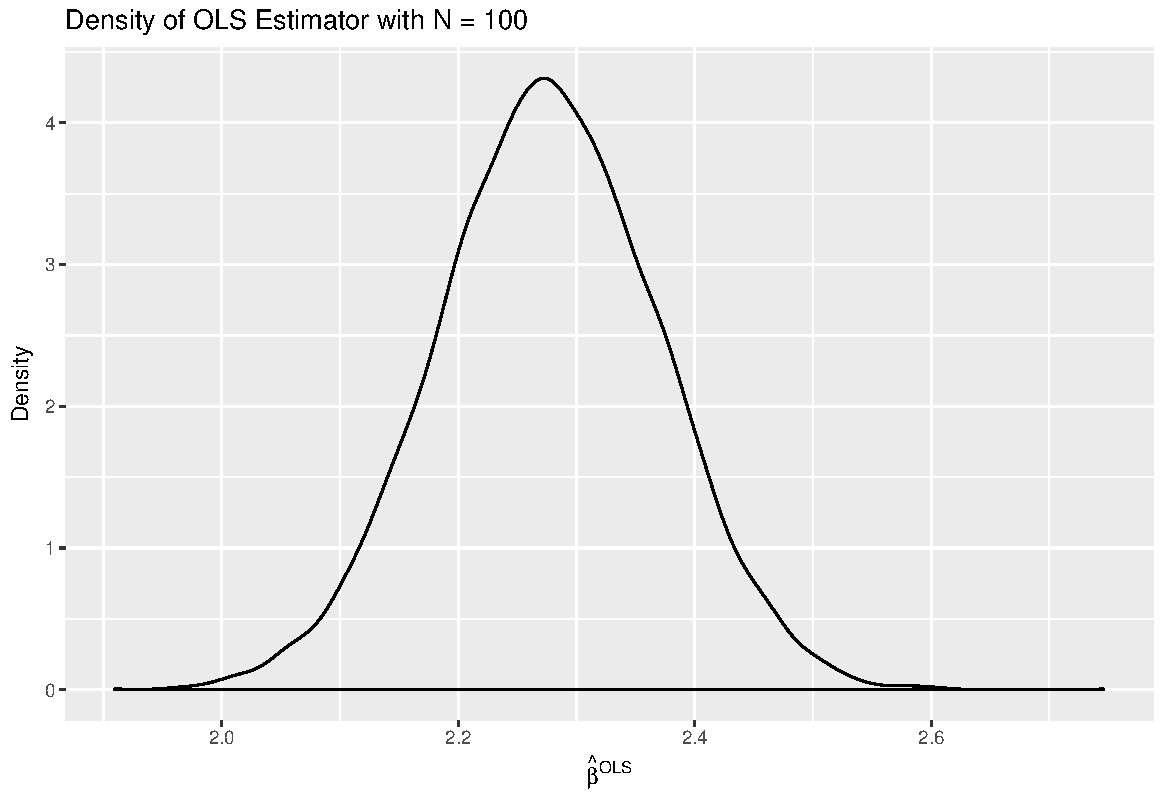
\includegraphics[width=.3\textwidth]{ols_smallN.pdf}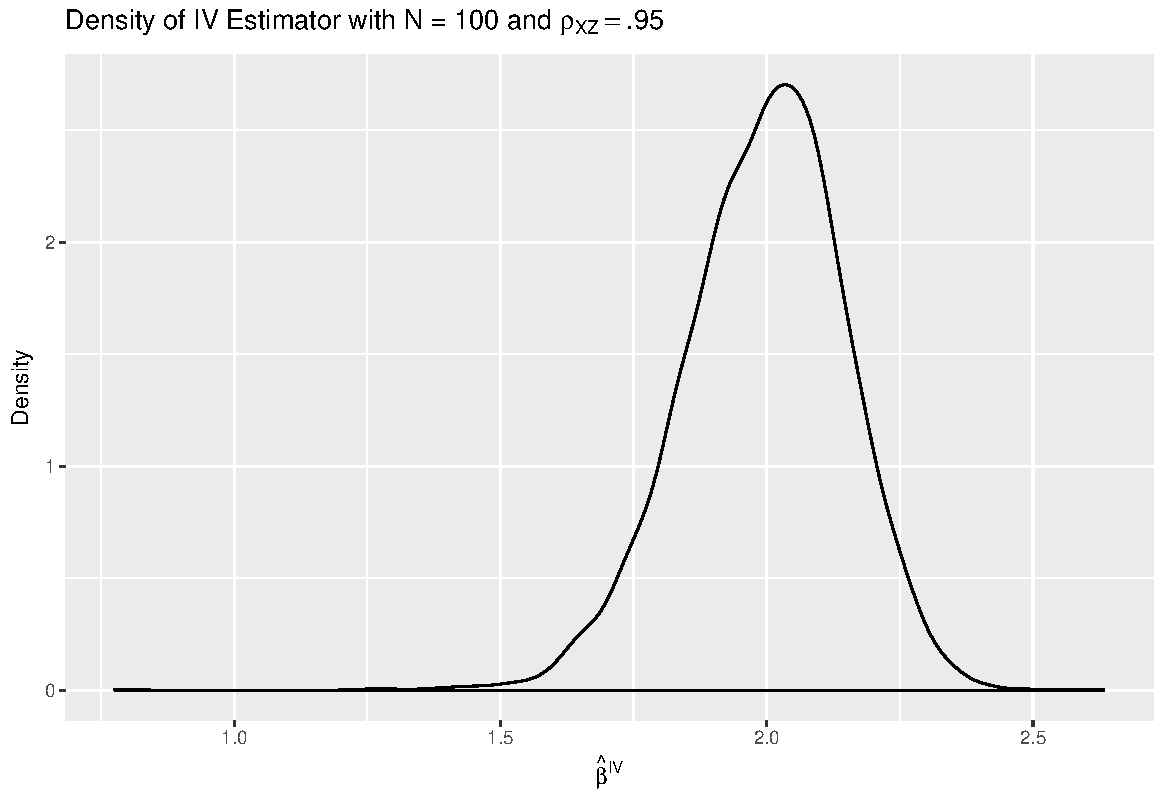
\includegraphics[width=.3\textwidth]{strongIV_smallN.pdf}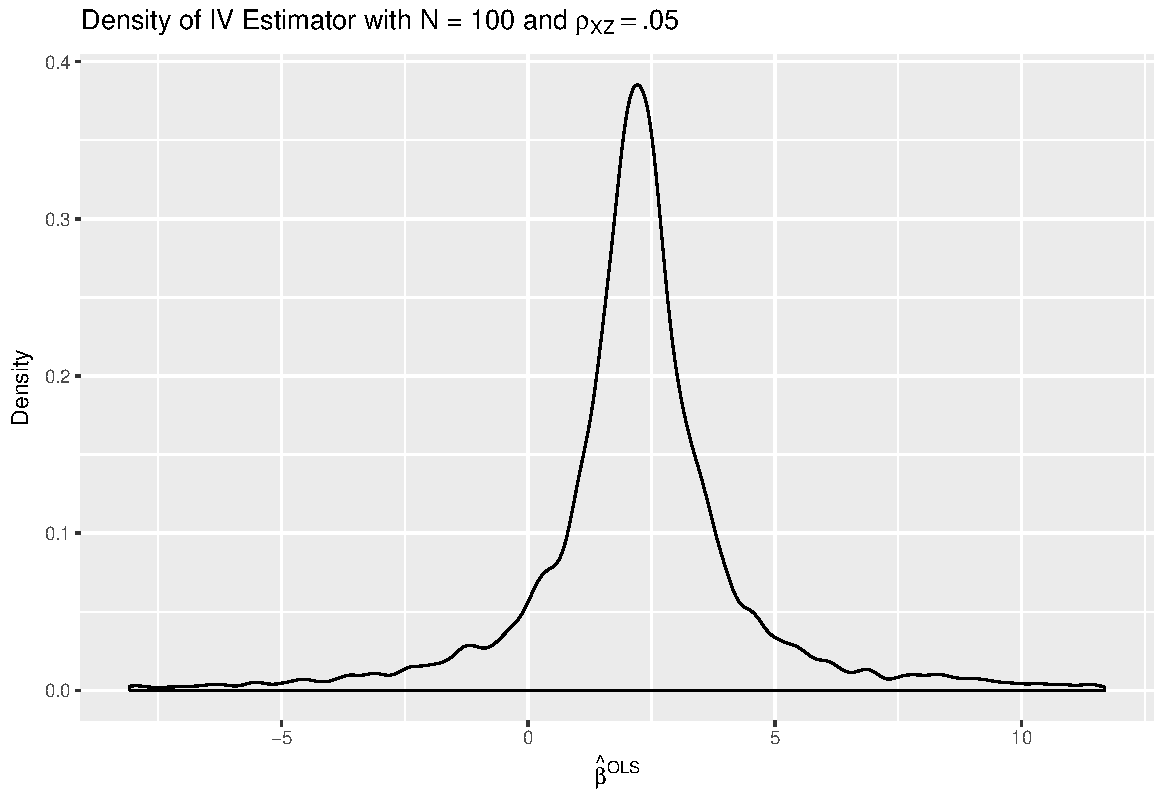
\includegraphics[width=.3\textwidth]{weakIV_smallN.pdf}
\end{figure}

\begin{itemize}{\footnotesize
\item OLS is biased with $\mu=2.27$ and $\sigma^2=.008$
\item Strong IV is unbiased (asymptotically) with $\mu=1.99$ and $\sigma^2 = .024$
\item Weak IV is unbiased (asymptotically) with $\mu=2.05$ but $\mathbf{\sigma^2 = 1653.11}$

}
\end{itemize}


\end{frame}



\begin{frame}{The Sampling Distribution of $\hat\beta$}
\[
	Y = 1 + 2 X + \varepsilon
\]

\begin{figure}
\centering \caption{\small Distribution of $\hat\beta$ for OLS, weak IV, strong IV with $N=10000$}
	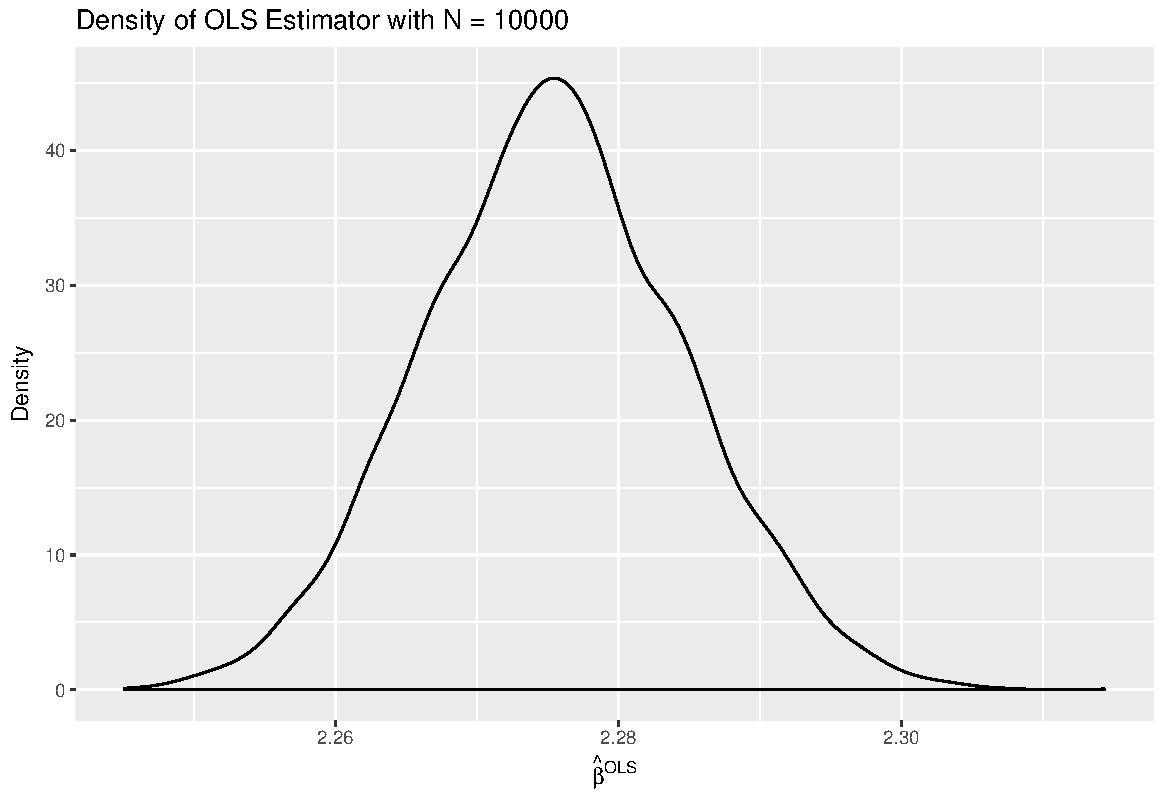
\includegraphics[width=.3\textwidth]{ols_largeN.pdf}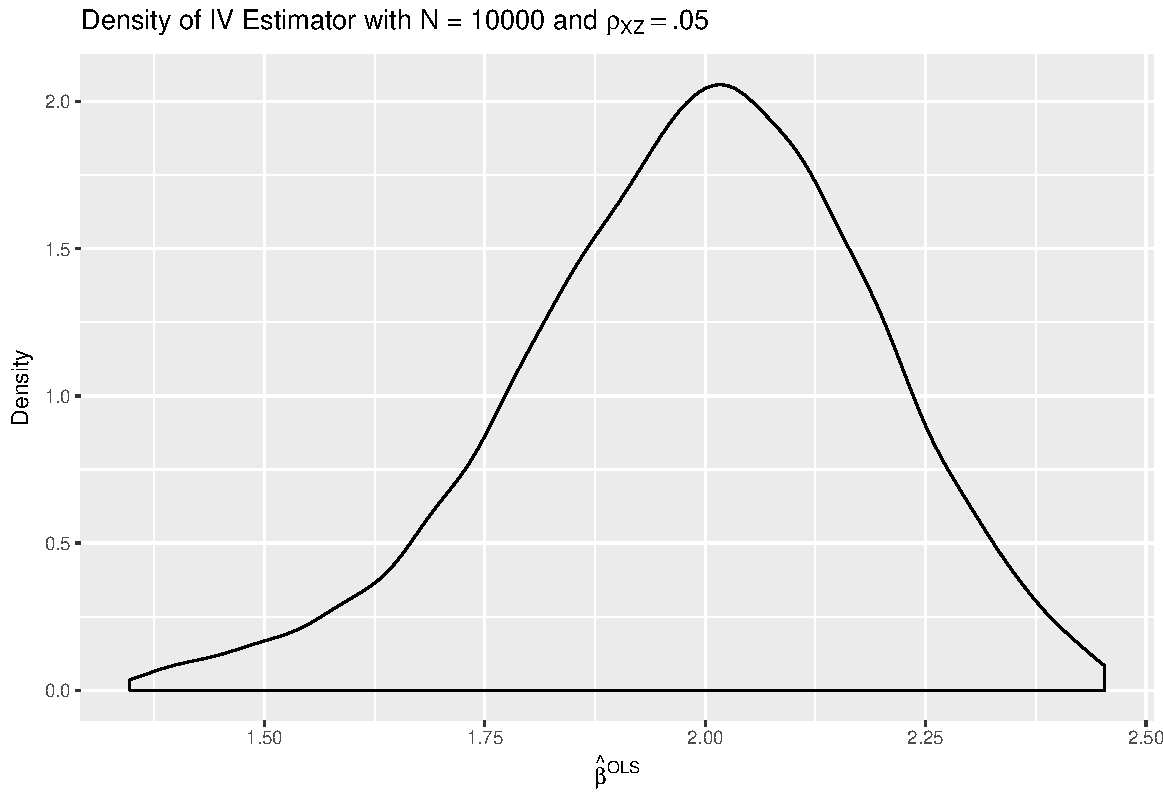
\includegraphics[width=.3\textwidth]{weakIV_largeN.pdf}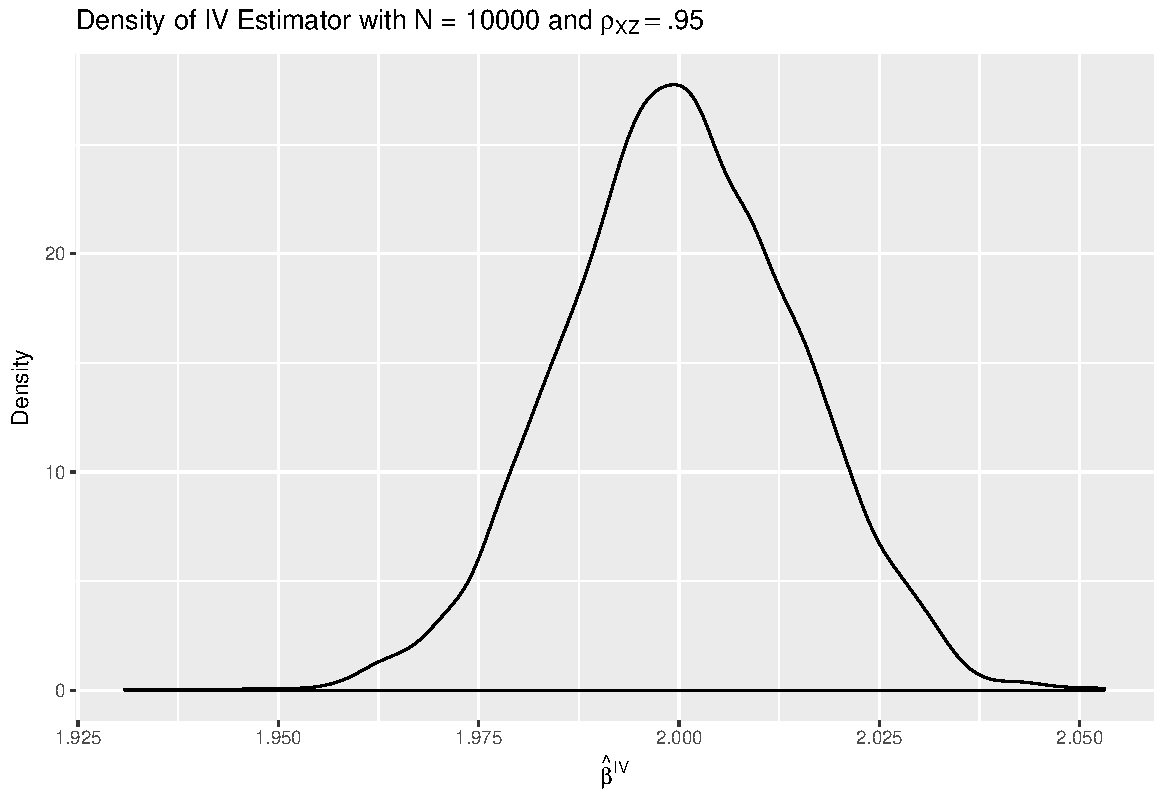
\includegraphics[width=.3\textwidth]{strongIV_largeN.pdf}
\end{figure}

\begin{itemize}{\footnotesize
\item OLS remains biased with $\mu=2.28$ and $\sigma^2=.000085$
\item Strong IV is consistent with $\mu=1.99$ and $\sigma^2 =.00021$
\item Weak IV is consistent with $\mu=2.05$ and even with $N=10k$, $\sigma^2 = .05$
	\begin{itemize}{\scriptsize
		\item Still over 100x larger variance than strong instruments!

	}
	\end{itemize}

}
\end{itemize}


\end{frame}


\begin{frame}{What is the Danger of the CLT Failing?}

	\begin{itemize}
		\item With weak IV, CLT fails and behaves poorly even if $N$ is large
		\item Remember that for testing we want to reject the null hypothesis incorrectly 5\% of the time
			\begin{itemize}
				\item When the CLT fails, our trusty 1.96 critical value is way off base
				\item Example rejection probabilities for test that $\hat\beta=2$
				\begin{table}[H]
				\centering
				\begin{tabular}{rr}
						{\bf Hypothetical Situation} & $P(|t|>1.96)$ \\
						Weak IV, $N=100$ &  0.3\% \\
						Strong IV, $N=100$ & 4.2\% \\
						Weak IV, $N=10000$ & 3.2\% \\
						Strong IV, $N=10000$ & 5.1\% \\
				\end{tabular}
				\end{table}
				\item Goal should be 5\% but for weak IV with $N$ small, almost never reject; still only 3\% even for $N$ large---this is a bad test!

			\end{itemize}
	\end{itemize}


\end{frame}


\begin{frame}{Checking The IV Assumptions II}

\begin{itemize}
\item The two major assumptions:
\begin{enumerate}
	\item Relevance: $Cov(X,Z)\ne 0$, or that $E\left[{\bf z}_i {\bf x}_i' \right]$ has full rank

	\item Exogeneity: All instruments must be uncorrelated with $\varepsilon$
\end{enumerate}
\smallskip
	\item Now, let's talk about the exogeneity assumption.
	\item With one IV, it's impossible to test exogeneity, hence
	the need to evaluate exogeneity by thinking about whether
	some unobserved variables might be correlated with the instrument.
	\item With extra instruments, we can test the IVs against each other.
	Similarly, one IV allows us to test the validity of OLS.
	\item In all cases, the most we can do is test one exogeneity assumption
	against another, we can never test the validity of an exogeneity assumption on its own.


\end{itemize}
\end{frame}

\begin{frame}{Overidentification}
\begin{itemize}
	\item When the number of regressors equals the number of instruments,
	the model is {\bf just identified}. When there are
	more instruments than regressors, the model is {\bf overidentified}.

	\medskip
	\item For a just identified model, the 2SLS estimator simplifies to\[
	\mathbf{b}_{IV}=\left(\mathbf{Z}'\mathbf{X}\right)^{-1}\mathbf{Z}'\mathbf{y},
	\]
	which is often called simply the {\bf IV estimator}.

	\medskip
%	\item (Derivation on board)

\end{itemize}
\end{frame}

\begin{frame}{A Note on Moments I}
\begin{itemize}
	\item Recall the property of the OLS estimator:\[
\mathbf{X}'\mathbf{e}_{OLS}=\mathbf{0}
\]
where
\begin{align*}
\mathbf{e}_{OLS}=\left(\mathbf{y}-\mathbf{X}\mathbf{b}_{OLS}\right)
\end{align*}
	\item Similarly, for the IV estimator,
\begin{align*}
\mathbf{Z}'\mathbf{e}_{IV}= \mathbf{0}
\end{align*}
where
\begin{align*}
\mathbf{e}_{IV}=\left(\mathbf{y}-\mathbf{X}\mathbf{b}_{IV}\right)
\end{align*}
	\item (Derivation on board)

\end{itemize}
\end{frame}

\begin{frame}{A Note on Moments II}
\begin{align*}
\mathbf{X}'\mathbf{e}_{OLS} &=\mathbf{0} \\
\mathbf{Z}'\mathbf{e}_{IV} &= \mathbf{0}
\end{align*}
\begin{itemize}
	\item A consequence of this is that we can't
	test the assumption that the instrument(s) and
	error terms are uncorrelated by looking at the
	correlation between the instrument(s) and residuals.

	\smallskip
	\item Similarly, the residuals from OLS don't allow
	us to test whether the error terms are correlated with the
	regressors.

	\smallskip
	\item However, the residuals from IV can be used to test
	the OLS exogeneity assumption. Similarly, if we have
	more instruments than we need (overidentification),
	we can test the instruments against each other.


\end{itemize}
\end{frame}



\begin{frame}{Wu-Hausman Test}
\begin{itemize}
	\item Is OLS biased? Does the use of instrumental variables really make a difference in results?

	\smallskip
	\item Intuition: we can compare the OLS and IV coefficient estimates, see if they're different.
	If they differ and we believe in the validity of the IV, that's evidence that OLS is biased
	because of an endogenous regressor.

	\smallskip
	\item The Wu-Hausman test implements this idea formally. It can be derived
as a Wald test using the IV and OLS regression results, and it can
also be implemented using the following regression:
\begin{align*}
\boldsymbol{y=}\boldsymbol{X}\boldsymbol{\beta}+\hat{\boldsymbol{X}}\boldsymbol{\gamma}+\boldsymbol{\varepsilon}^{*}
\end{align*}
 where $\hat{\boldsymbol{X}}$ are the fitted values of $\boldsymbol{X}$
from the first-stage regression of $\boldsymbol{X}$ on $\boldsymbol{Z}.$

\smallskip
\item Testing $\boldsymbol{\gamma}=0$ is
\href{http://eclr.humanities.manchester.ac.uk/index.php/IV_in_R\#Testing_for_exogeneity}{one way}
of implementing the Hausman test. It can also be implemented using the
\href{https://stats.stackexchange.com/questions/134789/interpretation-of-ivreg-diagnostics-in-r}{AER package}.
\end{itemize}
\end{frame}




\iffalse
\begin{frame}[fragile]\frametitle{Example in \texttt{R}: Checking Angrist \& Evans Validity}
{\small
		\begin{lstlisting}[frame=single]  % Start your code-block
		gross
 # First Stage Test in Angrist & Evans
flm1 = lm(morekids ~ samesex + black + hispan, data=babyData)
lh1 = linearHypothesis(flm1,c("samesex"),vcov=vcovHC(flm1, type = "HC1"))

# First Stage Test in AE w/ Multiple Instruments
flm2 = lm(morekids ~ boyBoy + girlGirl + black + hispan, data=babyData)
lh2 = linearHypothesis(flm2,c("boyBoy","girlGirl"),vcov=vcovHC(flm2, type = "HC1"))
	\end{lstlisting}
\vspace{3mm}
	Results:
\begin{itemize}
	\item With ``Same Sex": $F = 1414.252$
	\item With ``BoyBoy" and ``GirlGirl": $F = 714.86$
\end{itemize}}
\end{frame}
\fi

\begin{frame}{Checking Instrument Validity II}
Exogeneity Assumption:
	\[
		Corr(Z_i,\varepsilon_i) \hspace{5mm} \text{for all }Z
	\]

	\begin{itemize}
		\item If exogeneity violated then $\hat X$ from the first stage will still be correlated with $\varepsilon\Rightarrow$
		omitted variables bias
		\item Usual case: need to \emph{assume} exogeneity
		\item With multiple instruments can [with some limitations] test exogeneity
			\begin{itemize}
				\item Intuition: if $Z^{(1)}$ and $Z^{(2)}$ are both valid instruments then using them separately should produce the same value of $\hat\beta$
				\item If $\hat\beta$ different for different $Z$'s then one $Z$ must be bad
			\end{itemize}
	\end{itemize}
\end{frame}

\begin{frame}{Operationalizing the Intuition}{Defining the $J$ Statistic}

	\begin{itemize}
		\item Procedure to Test Overidentifying Restrictions
			\begin{enumerate}
				\item Estimate the model using 2SLS
				\item Compute $e_i$ with $X_i$ (not $\hat X_i$):
					\[
						e_i = Y_i - \hat\beta_0 - \hat\beta_1 X_i^{(1)} - ... \hat\beta_m X_i^{(k)}
					\]
				\item Regress $e_i$ on all $Z$'s and exogenous variables:
				\[
					e_i = \alpha_0 + \alpha_1 Z_i^{(1)} + ... +\alpha_m Z_i^{(m)} +  Exogenous + \varepsilon_i
				\]
				\item Compute the $F$ statistic for $\alpha_1=...=\alpha_m=0$ but do \emph{not} do the standard $F$ test
(degrees of freedom would be wrong)
				\item Compute $J = mF$, where $m$ is the number of instruments
			\end{enumerate}

	\end{itemize}
\end{frame}


\begin{frame}{Operationalizing the Intuition}{Performing the $J$ Test}
\begin{itemize}
		\item Under the null hypothesis, $J\sim \chi^2_{m-k}$, where $k$ is the number of regressors.
			\begin{itemize}
				\item Notice: We use $m-k$ degrees of freedom, not $m$
				\item Why? Because $e$ is a function of $\hat\beta$, which has $k$ parameters
				\item If at least one $\alpha\ne 0$ then at least one instrument is endogenous
			\end{itemize}
		\item The $J$-test:
			\begin{itemize}
				\item Calculate the $J$ statistic
				\item Compare the $J$ statistic to the critical value for a $\chi^2_{m-k}$ distribution
				\item Instruments are not exogenous if the test is rejected (so we want the null to not be rejected)
			\end{itemize}
		\item This is know as Sargan's $J$ test, and it can be implemented using the
		\href{https://stats.stackexchange.com/questions/134789/interpretation-of-ivreg-diagnostics-in-r}{AER package}.
		\item We can only do this if over-identified
			\begin{itemize}
				\item If exactly identified, then $Cov(e,Z)=0$ as we argued above
			\end{itemize}
\end{itemize}
\end{frame}


\begin{frame}{Interpreting $J$ Test Results}

\begin{itemize}
		\item What happens if we reject the null?
			\begin{itemize}
				\item The $\alpha$ that is non-zero does not necessarily indicate the problematic instrument
				-- $e$ is itself not unbiased if IV assumptions violated
				\item Need to think hard about which instruments may be invalid
			\end{itemize}
		\item What happens if we do not reject the null?
			\begin{itemize}
				\item None of your instruments contradict each other by predicting very different $e$'s
				\item Does NOT imply that instruments must be valid---they could all be invalid 

			\end{itemize}
\end{itemize}

\end{frame}

\iffalse
\begin{frame}[fragile]\frametitle{Example in \texttt{R}: Angrist \& Evans}
{\scriptsize
\begin{itemize}
	\item Instruments: $Boy,Boy$ or $Girl,Girl$
	\item Endogenous regressor: $Three\_Children$
\end{itemize}
\begin{lstlisting}[frame=single]  % Start your code-block
		gross
# Run the Regression
m6 = ivreg(workedm ~ morekids | boyBoy + girlGirl, data=babyData)

# Back out the residuals
babyData$uHat = babyData$workedm - fitted(m6)

# Regress instruments on residual
jReg = lm(uHat ~  boyBoy + girlGirl, data=babyData)

# Back out the F-statistic on the instruments
jlh = linearHypothesis(jReg,c("boyBoy","girlGirl"),vcov=vcovHC(jReg, type = "HC1"))

# Don't forget to multiply by number of instruments!
Jstat = 2*jlh$F[2]
\end{lstlisting}}
\end{frame}
\fi


\begin{frame}{Simultaneous Equations Models}

New Model:
\begin{align*}
	Y_i = \beta_0 + \beta_1 X_i + \varepsilon_i\\
	X_i = \alpha_0 + \alpha_1 Y_i + \nu_i
\end{align*}

\begin{itemize}
	\item In many economic environments, variables both determine each other ``in equilibrium" or are determined together ``jointly"
	\item A model where $X$ and $Y$ ``cause" each other	is called a {\bf simultaneous equations model}
	\item Examples:
		\begin{itemize}
			\item Angrist \& Evans is an example of this: labor supply and fertility decisions are determined jointly, there is no one-way channel
			\item Supply and demand is the canonical example: supply equations and demand equations are of interest but in equilibrium only observe $Q_S=Q_D$
			\item Also common in macroeconomic contexts: interest rates, unemployment rates, etc.
		\end{itemize}
	%\item We will usually assume that $Cov(\varepsilon,\nu)=0$
\end{itemize}

\end{frame}

\begin{frame}{Simultaneity Bias}

{\small
Direct effect of $X$ on $Y$:
\[
	Y_i = \beta_0 + \beta_1 X_i + \varepsilon_i
\]

\vspace{2mm}

\only<1>{
\noindent First let's solve for $X$ and $Y$ \emph{jointly}

\begin{eqnarray*}
	X_i & = & \alpha_0 + \alpha_1 Y_i + \nu_i\\
		& = & \alpha_0 + \alpha_1 (\beta_0 + \beta_1 X_i + \varepsilon_i) + \nu_i\\
		& = & \alpha_0 + \beta_0\alpha_1 + \alpha_1\beta_1 X_i + \alpha_1 \varepsilon_i + \nu_i
\end{eqnarray*}

Which implies...
\[
	X_i = \frac{\alpha_0 + \alpha_1\beta_0 + \nu_i}{1-\alpha_1\beta_1} + \underbrace{\frac{\alpha_1}{1-\alpha_1\beta_1}\times \varepsilon_i}_{OVB}
\]

}

\only<2-4>{
\noindent What happens with OLS? Think about the OVB equation:

\begin{eqnarray*}
	\hat\beta_1^{OLS} &\to & \beta_1 + \frac{Cov(X,\varepsilon)}{Var(X)}\\ 
					& = & \beta_1 + \frac{Cov\left(\frac{\alpha_0 + \alpha_1\beta_0 + \nu_i}{1-\alpha_1\beta_1} + \frac{\alpha_1}{1-\alpha_1\beta_1}\times \varepsilon_i,\varepsilon_i\right)}{Var\left(\frac{\alpha_0 + \alpha_1\beta_0 + \nu_i}{1-\alpha_1\beta_1} + \frac{\alpha_1}{1-\alpha_1\beta_1}\times \varepsilon_i\right)}\\ 
					& = & \beta_1 + \frac{\frac{\sigma_{\varepsilon\nu} + \alpha_1 \sigma^2_\varepsilon}{1-\alpha_1\beta_1}}{\frac{\sigma^2_\nu +\alpha_1^2\sigma^2_\varepsilon + 2\alpha_1\sigma_{\varepsilon\nu}}{(1-\alpha_1\beta_1)^2}}\\
					& = & \beta_1 + (1-\alpha_1\beta_1)\times\frac{\alpha_1\sigma^2_\varepsilon + \sigma_{\varepsilon\nu}}{\alpha_1^2\sigma^2_\varepsilon + \sigma^2_\nu + 2\alpha_1 \sigma_{\varepsilon\nu}}
\end{eqnarray*}

}
}

\end{frame}

\begin{frame}{Understanding Simultaneity Bias}

OLS with Simultaneity:
\[
	\hat\beta_1^{OLS} \to \beta_1 + (1-\alpha_1\beta_1)\times\frac{\alpha_1\sigma^2_\varepsilon + \sigma_{\varepsilon\nu}}{\alpha_1^2\sigma^2_\varepsilon + \sigma^2_\nu + 2\alpha_1 \sigma_{\varepsilon\nu}}
\]

Consider the special case that $\varepsilon$ and $\nu$ are independent:
\[
	\hat\beta_1^{OLS} = \beta_1 \frac{\sigma^2_\nu}{\sigma^2_\nu + \alpha_1^2\sigma^2_\varepsilon} + \frac{1}{\alpha_1} \frac{\alpha_1^2\sigma^2_\varepsilon}{\sigma^2_\nu + \alpha_1^2 \sigma^2_\varepsilon}
\]

\begin{itemize}
	\item OLS becomes a weighted average of two pieces:
		\begin{enumerate}
			\item $\beta_1$: the effect of $X$ on $Y$
			\item $1/\alpha_1$: the feedback loop from $Y$ to $X$ back to $Y$
		\end{enumerate}
 	\item This is {\bf simultaneity bias}

\end{itemize}


\end{frame}

\begin{frame}{IV Can Solve Simultaneity Bias}

Why cover simultaneity bias \emph{now}?

\vspace{3mm}

New Model:
\begin{align*}
	Y_i =& \beta_0 + \beta_1 X_i + \varepsilon_i\\
	X_i =& \alpha_0 + \alpha_1 Z_i + \alpha_2 Y_i + \nu_i
\end{align*}

\begin{itemize}
	\item If we have data on $Z$, we can potentially use $Z$ as an instrument!
	\item What conditions would $Z$ have to fulfill?
		\begin{enumerate}
			\item Instrument Relevance: $\alpha_1>0$
			\item Instrument Exogeneity: $Cov(Z_i,\varepsilon_i)=0$
		\end{enumerate}

\end{itemize}

\end{frame}



\begin{frame}{Example: Angrist \& Evans}

Model:
\begin{align*}
Hours_i =& \beta_0 + \beta_1 Children_i + \varepsilon_i\\
Children_i =& \alpha_0 + \alpha_1 Hours_i + \alpha_2 SameSex_i + \nu_i
\end{align*}

\begin{itemize}
	\item $SameSex$: indicator for whether first two children have same sex
	\item Hours and children are determined jointly
	\item Also $Cov(\varepsilon,\nu)$ is unlikely to be 0
		\begin{itemize}{\footnotesize
			\item Education can matter for both number of children and hours worked (so education is part of $\varepsilon$ and $\nu$)
			\item Being married may matter for both
			\item Quality of non-financial benefits (e.g., maternity leave)

			}
		\end{itemize}
	\item So formally, the instrument $SameSex$ is supposed to help solve simultaneity
\end{itemize}
\end{frame}


\begin{frame}{Example: Angrist \& Evans}
\begin{center}
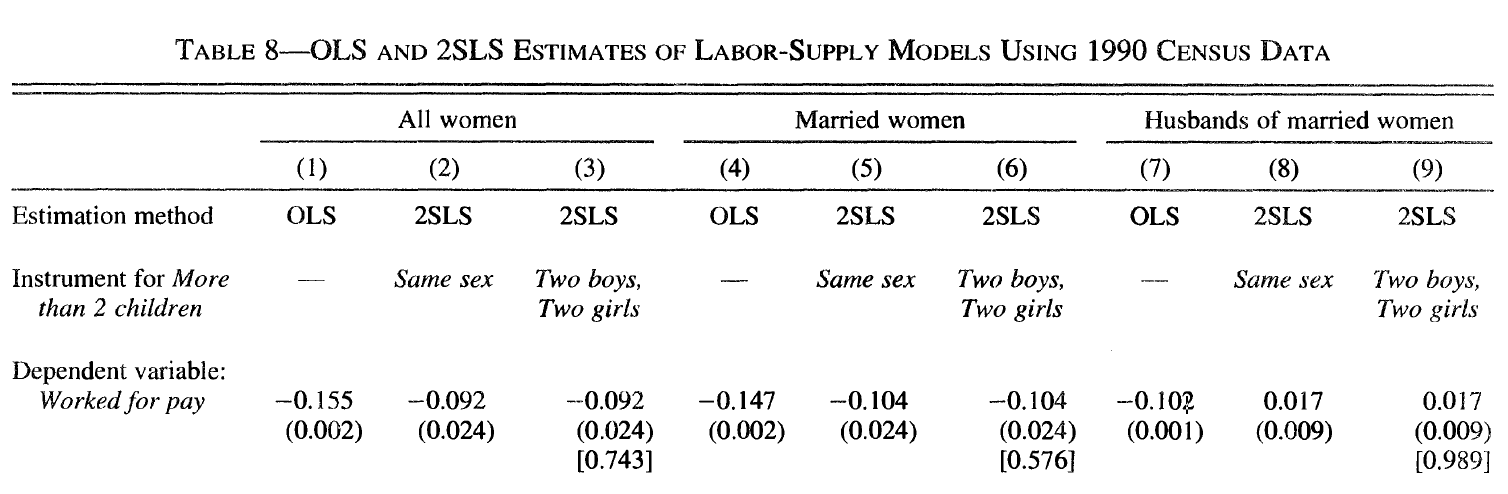
\includegraphics[scale=.45]{AE_tab8}
\end{center}
\end{frame}


\begin{frame}{Example: Porter (1983)}
\begin{itemize}
	\item The Joint Executive Committee's (19th Century railroad cartel)
	main business was transporting grain from Midwest to ports on East Coast.

	\item Porter (1983) estimates the following simultaneous system:\[
\begin{array}{cccc}
\text{demand:} & \log Q_{t} & = & \alpha_{0}+\alpha_{1}\log P_{t}+\alpha_{2}L_{t}+U_{1t}\\
\\
\text{supply:} & \log P_{t} & = & \beta_{0}+\beta_{1}\log Q_{t}+\beta_{2}S_{t}+\beta_{3}I_{t}+U_{2t}
\end{array}
\]
where
\begin{itemize}
\item $Q_{t}$ is the quantity (tonnage of grain) transported by the JEC
\item $P_{t}$ is the price per ton of grain transported
\item $L_{t}$ is a dummy for whether the Great Lakes were open to navigation
\item $S_{t}$ is a vector of time dummies
\item $I_{t}$ is an indicator for whether the JEC was colluding
\end{itemize}
\end{itemize}
\end{frame}

\begin{frame}{Example: Porter (1983)}
\begin{align*}
	ext{demand:} & \log Q_{t} & = & \alpha_{0}+\alpha_{1}\log P_{t}+\alpha_{2}L_{t}+U_{1t}\\
\\
	ext{supply:} & \log P_{t} & = & \beta_{0}+\beta_{1}\log Q_{t}+\beta_{2}S_{t}+\beta_{3}I_{t}+U_{2t}
\end{align*}
\begin{align*}
	ext{demand:} & \log Q_{t} & = & \alpha_{0}+\alpha_{1}\log P_{t}+\alpha_{2}L_{t}+U_{1t}\\
\\
	ext{supply:} & \log P_{t} & = & \beta_{0}+\beta_{1}\log Q_{t}+\beta_{2}S_{t}+\beta_{3}I_{t}+U_{2t}
\end{align*}
\end{frame}
% \begin{align*}
% 	ext{demand:} & \log Q_{dt} & = & \alpha_{0}+\alpha_{1}\log P_{dt}+\varepsilon_{dt}\\
% \\
% 	ext{supply:} & \log Q_{st} & = & \beta_{0}+\beta_{1}\log P_{st}+\beta_{2}\omega_{t}+\varepsilon_{st}
% \end{align*}


\begin{frame}{Example: Roberts and Schlenker (2013)}
\begin{itemize}
	\item How much does the biofuels mandate increase the price of grains?
	It depends on supply and demand.

	\item Roberts and Schlenker (2013) estimate the following supply and demand equations:\[
\begin{array}{cccl}
\text{demand:} & \log Q_{dt} & = & \alpha_{0}+\alpha_{1}\log P_{dt}+\varepsilon_{dt}\\
\begin{align*}
\E\left[\boldsymbol{m}\left(y_i,\mathbf{x}_i;\boldsymbol{\theta}_0\right) \right]=0,
\end{align*}
where
\begin{itemize}
\item $Q_{st}$ is global grain supply (calories)
\item $Q_{dt}$ is global grain consumption ($Q_{st}\ne Q_{dt}$ because
of storage)
\item The prices are measured at different times (planting vs harvest time)
\item $\omega_{t}$ is a yield shock (due to weather), used as an instrument
for demand
\item $\omega_{t-1}$ is used as an instrument for supply (through storage,
past production matters for current prices)
\end{itemize}
\end{itemize}
\end{frame}

\begin{frame}{Example: Roberts and Schlenker (2013)}
\begin{center}
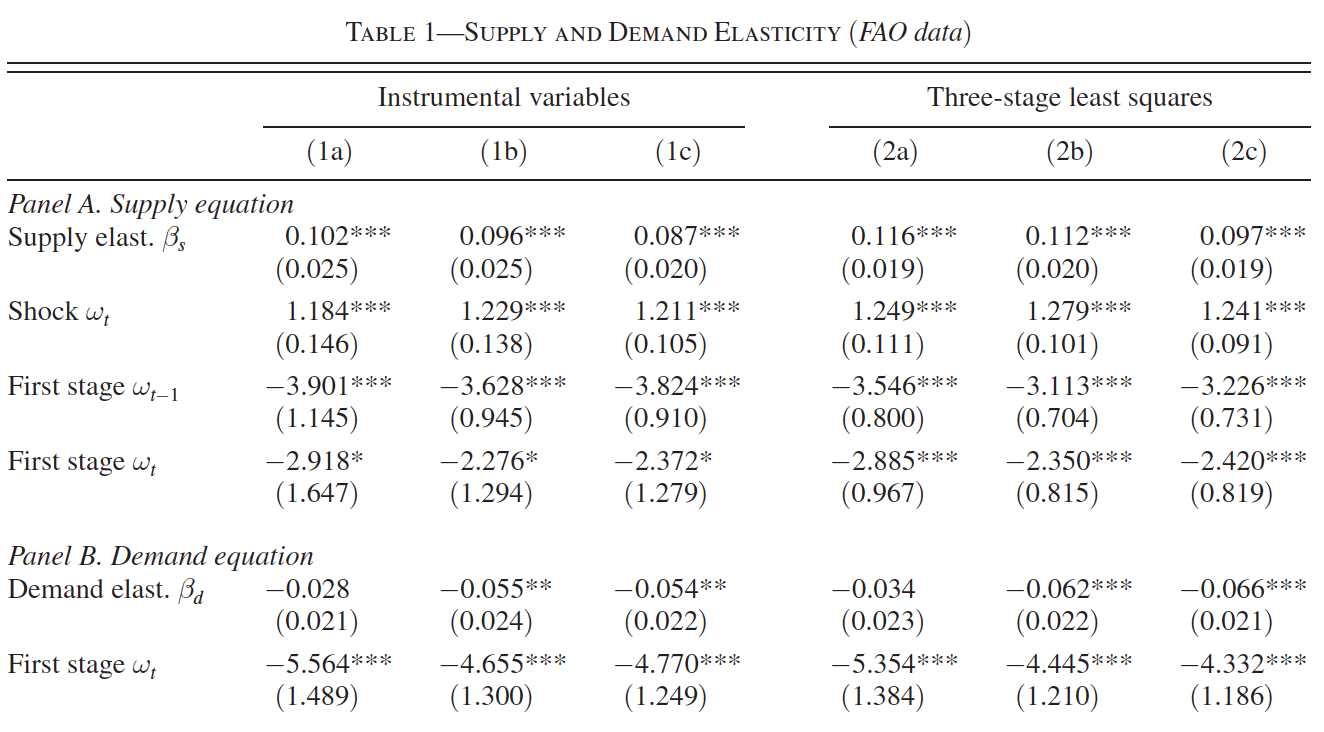
\includegraphics[scale=.5]{RS_t1}
\end{center}
\end{frame}



%\begin{frame}{More weather-based IVs}
%From \href{https://www.iaee.org/en/publications/ejarticle.aspx?id=2243}{Hughes, Knittel, Sperling (2008)}
%\begin{center}
%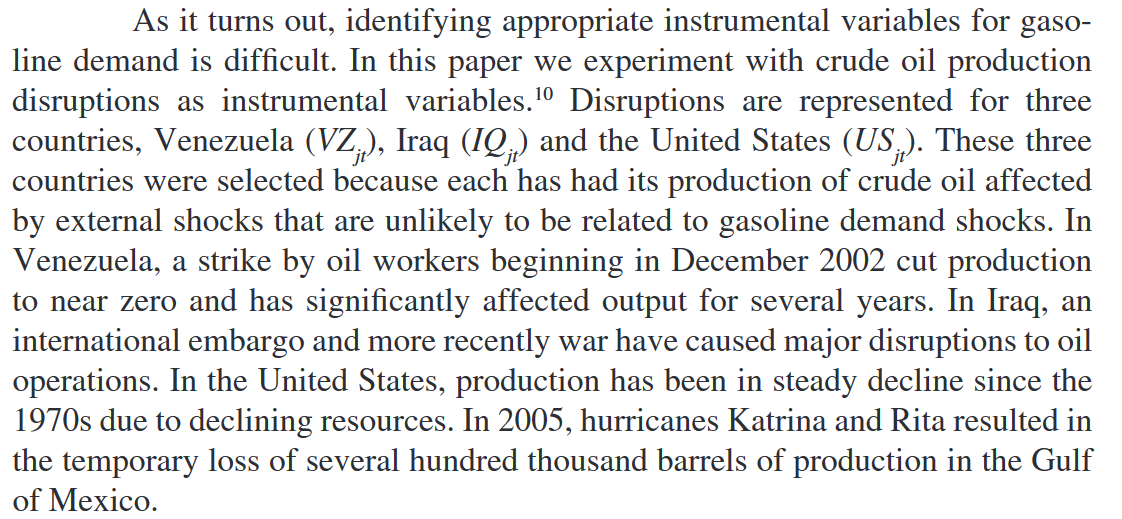
\includegraphics[width=.9\textwidth]{Katrina_iv}
%\end{center}
%\end{frame}



\begin{frame}{Simultaneity more examples}
\begin{itemize}
	\item \href{https://www.ptscott.com/papers/telecom_infrastructure.pdf}{Download speeds and mobile data consumption}:
		Consumers use their smart phones more when download speeds are fast, but high usage leads to congestion, which slows
		down speeds.

	\bigskip
	\item Road investment and travel demand: better roads are more appealing to travelers, and highly-used routes are likely
		to receive more funding .

	\bigskip
	\item Public opinion influences policy, and policy influences public opinion (cigarettes, parental leave, same-sex marriage). 

	\bigskip
	\item Intensity of policing and crime rates. 
\end{itemize}
\end{frame}



\begin{frame}{Measurement Error}

The problem: the $X$ variable is measured with noise

\begin{itemize}
	\item The idea mathematically:
		\begin{align*}
			\text{\bf{TRUTH}:} Y &= \beta_0 + \beta_1 X + \varepsilon \\
			\text{\bf{DATA}:}  Y &= \beta_0 + \beta_1 X^* + \varepsilon^*
		\end{align*}
		where $X^*$ is a noisy measure of $X$
	\item Examples: 
	\begin{itemize}
		\item Recording errors in data entry
		\item Recollection errors in survey data (these are frequent)
		\item Rounding errors
		\item Hard to measure variables (e.g., a firm's capital stock)
	\end{itemize}
	\item Note: we can also have measurement error in $Y$. Turns out these behave differently
\end{itemize}

	
\end{frame}

\begin{frame}{Visualizing Measurement Error: Self-Reported Australian Incomes}
	
Survey question: What is your income in thousands? 

\begin{figure}[H]
	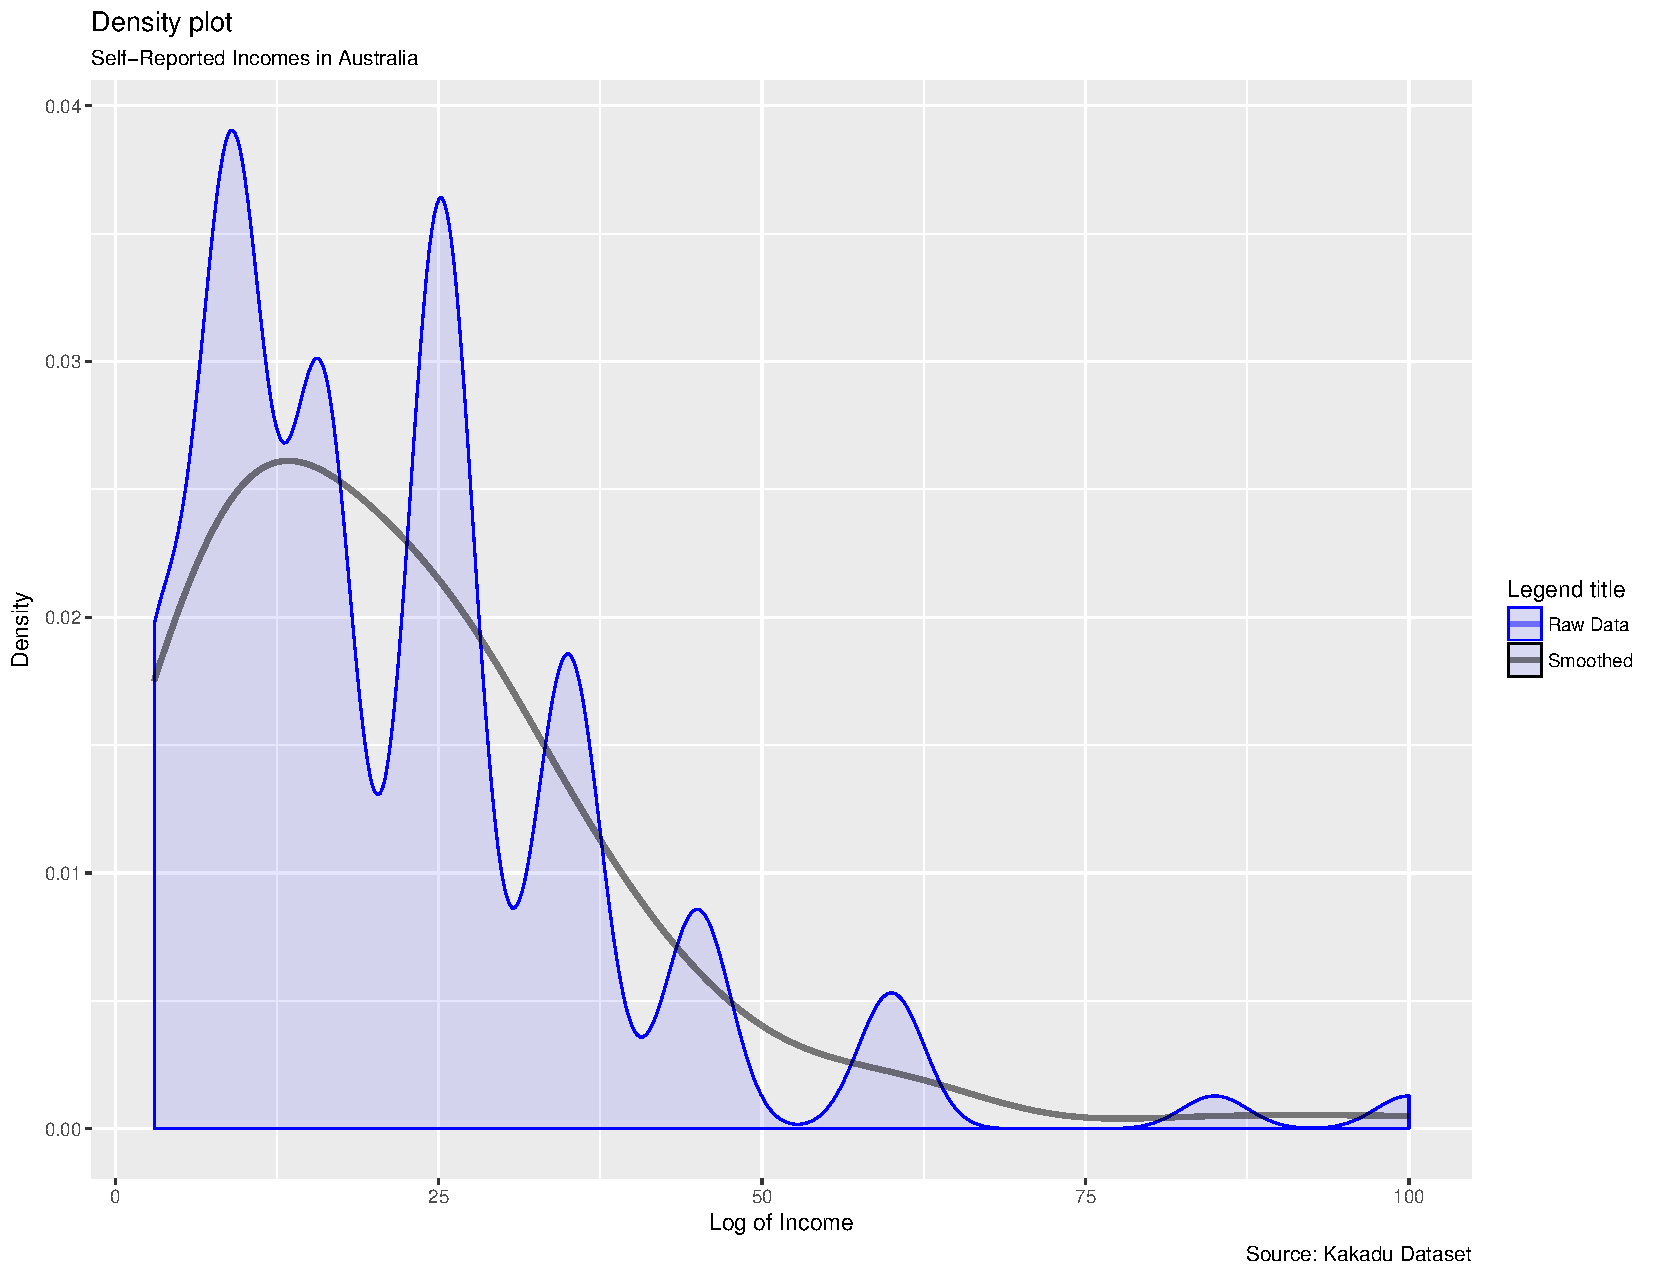
\includegraphics[width=.575\textwidth]{measurementErrorPlot.pdf}	
\end{figure}
	
	\begin{itemize}{\scriptsize
		\item The lumps occur at 5s and 0s
		\item E.g., people making 41k might say ``40" or ``45" instead of 41
			
		}
	\end{itemize}

	
\end{frame}

\begin{frame}{Measurement Error in $X$}{The Math of Measurement Error}

	
\begin{itemize}
	\item Consider adding and subtracting noise to the truth:
		\begin{align*}
			Y_i =& \beta_0 + \beta_1 X_i + \varepsilon_i\\
				=& \beta_0 + \beta_1 X_i^* + \underbrace{\beta_1(X_i - X_i^*) + \varepsilon_i}_{\text{``New" Error Term:} V_i}\\
				=& \beta_0 + \beta_1 X_i^* + V_i
		\end{align*}
	\item $X_i^*$ and $V_i$ likely to be correlated because $X^*$ is part of $V$
	\item Extra assumptions:
		\begin{itemize}
			\item {\bf Classical Errors-in-Variables:}
				\[
					X_i = X_i^* + u_i
				\begin{align*}
				n^{-1} \sum_{i=1}^n \boldsymbol{m}\left(y_i,\mathbf{x}_i;\boldsymbol{\theta}\right)
				\end{align*}
		\end{itemize}

\end{itemize}
	
	
\end{frame}


\begin{frame}{Measurement Error in $X$}{Classical Measurement Error}

Under classical measurement error:
	\[
		Y_i = \beta_0 + \beta_1 X_i^* + \underbrace{\beta_1u_i + \varepsilon_i}_{V_i}
	\]
\begin{itemize}
	\item Using the population definition of $\hat\beta^{OLS}$:{\small
		\begin{align*}
			\hat\beta^{OLS}\to & \frac{Cov(X^*,Y)}{Var(X^*)}\\
							=&\frac{Cov(X+u,\beta_0 + \beta_1 X + \varepsilon)}{Var(X+u)}\\
							=&\frac{Cov(X,\beta_0 + \beta_1 X + \varepsilon) + Cov(u,\beta_0 + \beta_1 X + \varepsilon)}{Var(X+u)}\\
							=& \frac{\beta_1 Cov(X,X) + 0}{Var(X+u)}
		\end{align*}}
		
		
\end{itemize}
	
	
\end{frame}

\begin{frame}{Measurement Error in $X$}{Classical Measurement Error, Cont'd}

\begin{itemize}
	\item Continuing from above:{\small
		\begin{align*}
			\hat\beta^{OLS}\to & \frac{\beta_1 Cov(X,X) + 0}{Var(X+u)}\\
							=& \beta_1\times\frac{Var(X)}{Var(X+u)}\\
							=& \beta_1\times\underbrace{\frac{\sigma^2_X}{\sigma^2_X + \sigma^2_u}}_{\text{Attenuation}}
		\end{align*}}
	\item Estimated coefficient converges to the truth times an attenuation term
		\begin{itemize}
			\item Attenuation term is less than 1 $\Rightarrow$ pushes coefficient towards zero
			\begin{itemize}
			\item {\bf NB:} It does \emph{not} make the term more negative---it dampens the coefficient and preserves the sign
			\end{itemize}
			\item This ``attenuates" the effect of $X$ on $Y$. Hence the name: {\bf attenuation bias}
		\end{itemize}
		
\end{itemize}
	
	
\end{frame}

\begin{frame}{Measurement Error in $X$}{Classical Measurement Error Intuition}	
	\begin{itemize}
		\item Why does measurement error attenuate the estimated effect of $X$ on $Y$?
		\begin{itemize}
			\item Noise in measured $X$ makes it more likely to see high $X$ and low $X$ with some $Y$ because of randomness
			\item Extreme example: fix $X$ and keep adding noise---eventually $X^*$ will look like noise itself
		\end{itemize}	
		\item Notice the following rearranging of the attenuation term:
			\[
				\frac{\sigma^2_X}{\sigma^2_X + \sigma^2_u} = \frac{1}{1+(\sigma^2_u/\sigma^2_X)}
			\]
			\begin{itemize}
				\item $\sigma^2_X/\sigma^2_u$ is called the {\bf signal-to-noise ratio}
				\item Larger signal to noise ratio $\Rightarrow$ smaller bias
				\item What matter is the \emph{relative} variance of $X$ to $u$
				\item If $\sigma^2_u$ is small \emph{relative} to $\sigma^2_X$ then attenuation bias isn't too large
			\end{itemize}
	\end{itemize}
\end{frame}

\begin{frame}{Visualizing Measurement Error}
	\begin{figure}[h]
	\only<1>{
		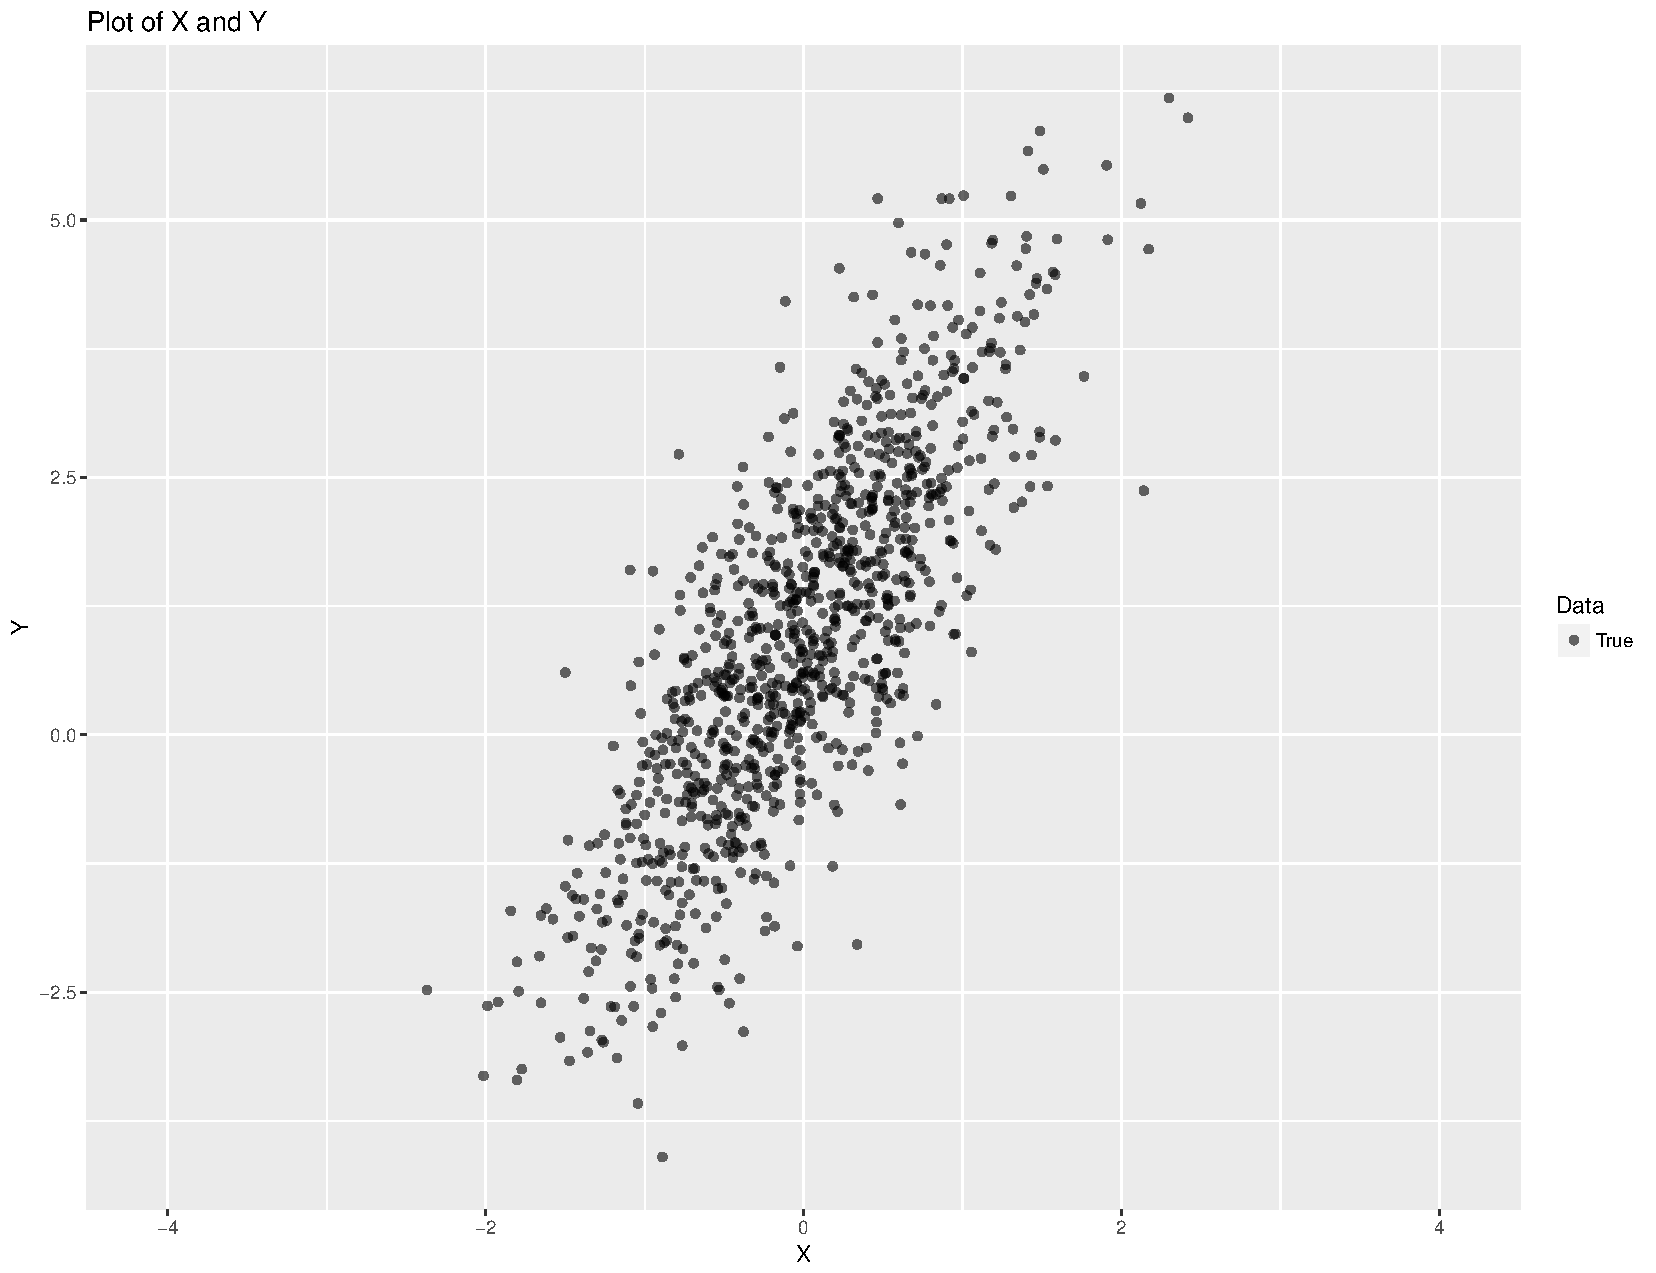
\includegraphics[width=.7\textwidth]{measurementErrorExample_1.pdf}
	}
	\only<2>{
		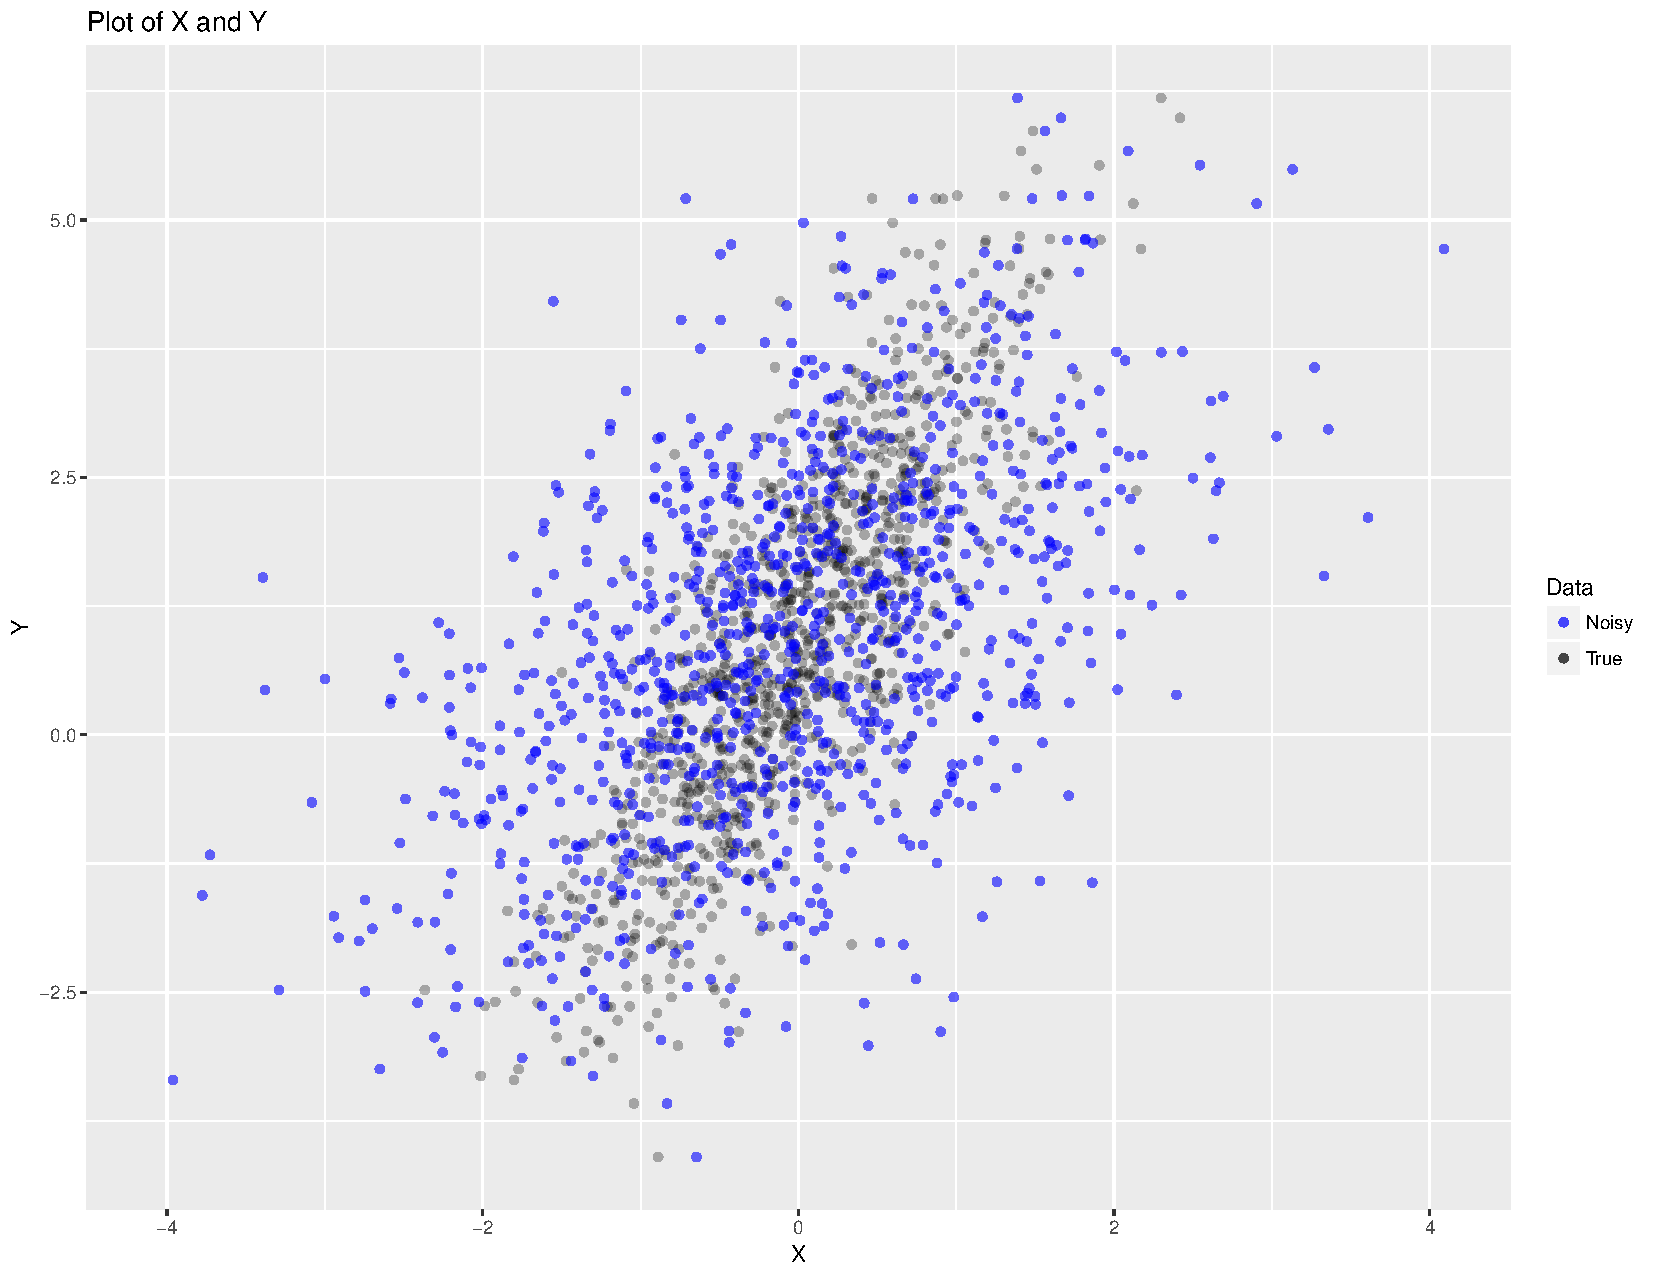
\includegraphics[width=.7\textwidth]{measurementErrorExample_2.pdf}
	}
	\only<3>{
		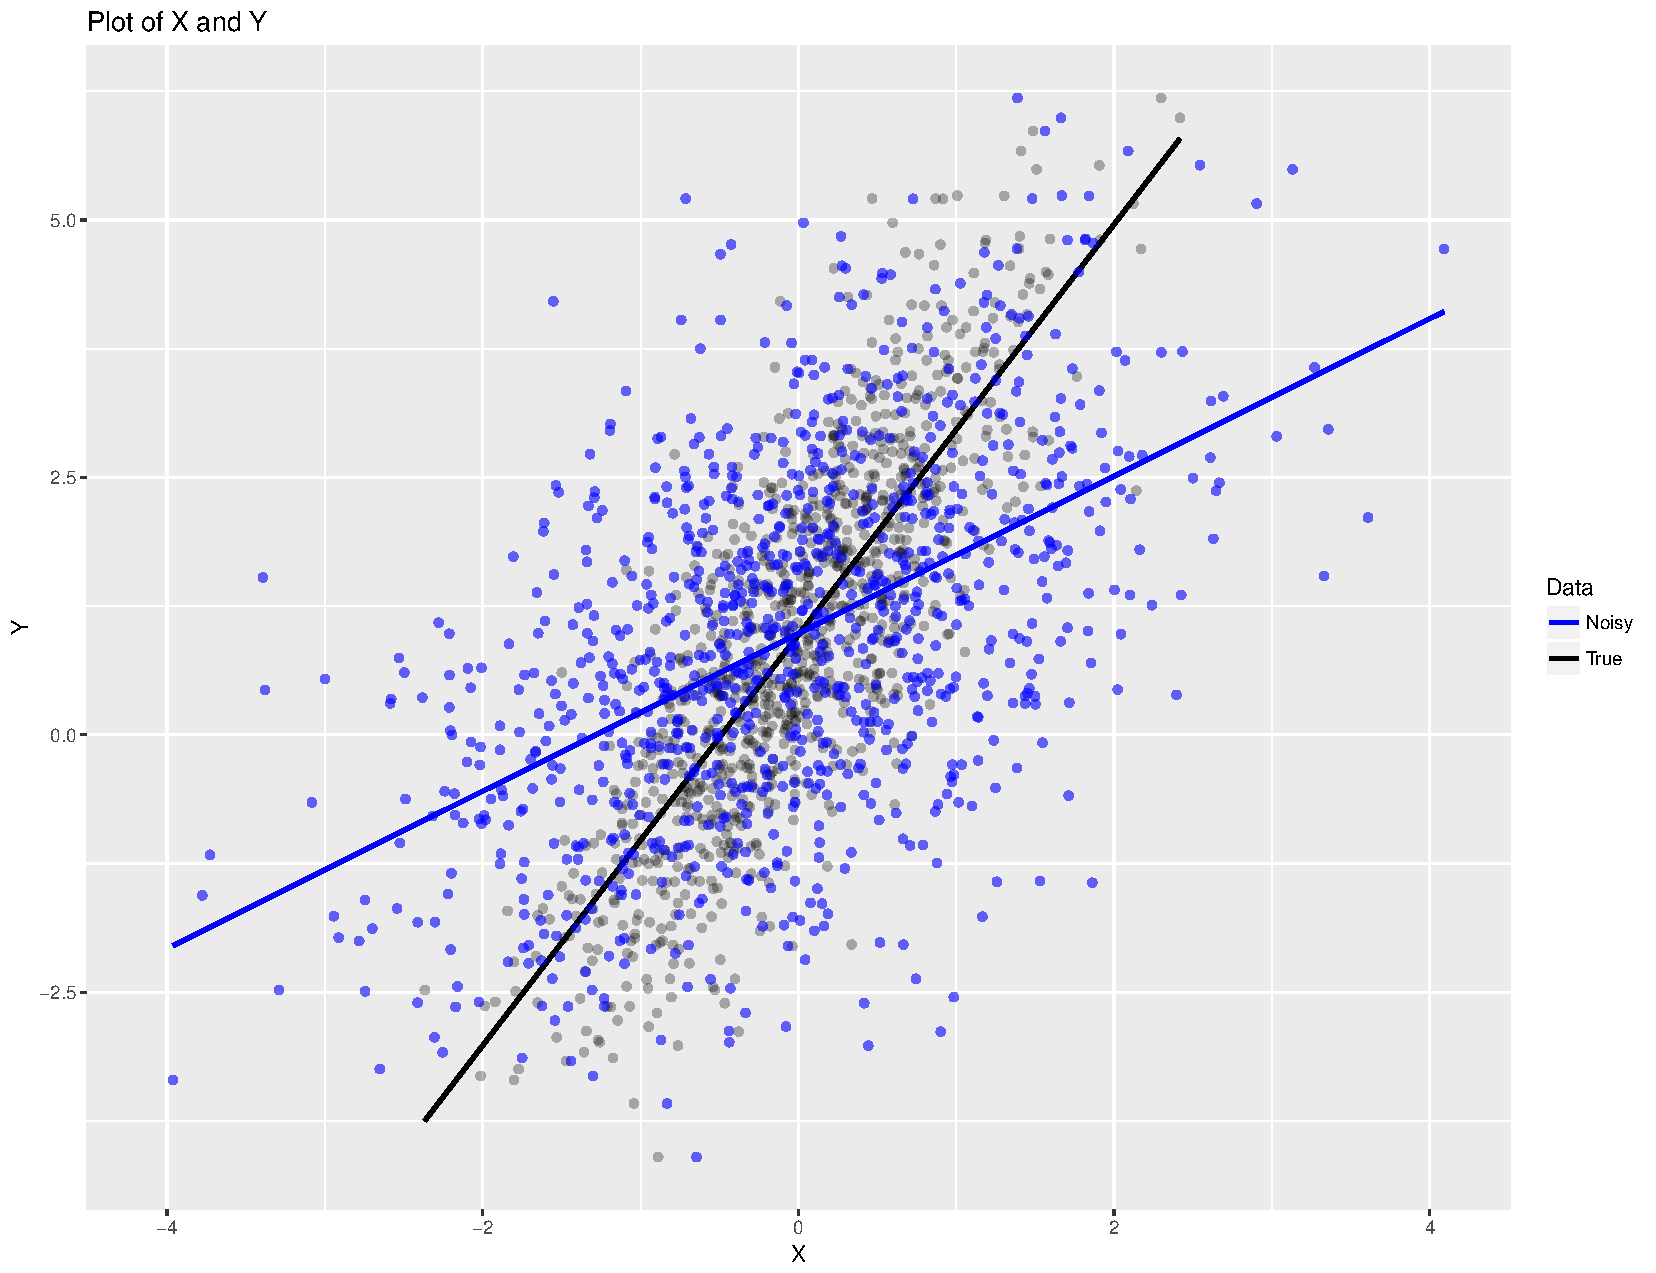
\includegraphics[width=.7\textwidth]{measurementErrorExample_3.pdf}
	}
	\end{figure}

	\begin{itemize}
		\only<1>{\item Suppose this is the true data. But...}
		\only<2>{\item ... you only observe the noisy data...}
		\only<3>{\item ... then what happens to the estimated slope?}
	\end{itemize}


\end{frame}





\begin{frame}{Measurement Error and IVs}
		\begin{align*}
			Y_i =& \beta_0 + \beta_1 X_i + \varepsilon_i\\
				=& \beta_0 + \beta_1 X_i^* + \underbrace{\beta_1(X_i - X_i^*) + \varepsilon_i}_{\text{``New" Error Term:} V_i}\\
				=& \beta_0 + \beta_1 X_i^* + V_i
		\end{align*}
\begin{itemize}
	\item How do we address attenuation bias using instrumental variables? 
% note we need something correlated with the measurement but not the measurement error; an independent
% measurement will do 		
\end{itemize}
\end{frame}



\begin{frame}{Measurement Error in $Y$}{No problemo}	
	\begin{itemize}
		\item Suppose the econometrician observes $Y^{*} = Y + u$, where $Y$ is the true value. \[
\begin{array}{ccl}
Y_{i} & = & \beta_{0}+\beta_{1}X_{i}+\varepsilon_{i}\\
Y_{i}+Y_{i}^{*} & = & \beta_{0}+\beta_{1}X_{i}+\varepsilon_{i}+Y_{i}^{*}\\
Y_{i}^{*} & = & \beta_{0}+\beta_{1}X_{i}+\varepsilon_{i}+\left(Y_{i}^{*}-Y_{i}\right)
\end{array}
\]
	\item Again, we can see this as changing the error term:
\[
Y_{i}^{*}=\beta_{0}+\beta_{1}X_{i}+V_{i}
\]
where $V_{i}=\varepsilon_{i}+\left(Y_{i}^{*}-Y_{i}\right).$	
		
		\item As long as this is classical measurement error, i.e. $E\left[u|X\right]= 0$,
		then as long as exogeneity is satisfied with the original error term $E\left[\varepsilon|X\right]=0$,
		it will still be satisfied for the modified error term $E\left[V|X\right]=0$.
		
\end{itemize}
\end{frame}		



\begin{frame}{IV as a method-of-moments estimator}
\begin{itemize}
	\item The Generalized Method of Moments includes everything we've
	done so far, and more.
	
	\item Recall how IV regression (just identified) results in residuals that satisfy\[
		{\bf Z}' 		{\bf e} = {\bf 0} .
	\]
	This is the sample analog of the population moment $E\left[ {\bf z}_i e_i \right]=0$.
	
	\medskip
	\item With a just identified model, the IV estimator is the unique estimator that sets 
	${\bf Z}' 		{\bf e} = {\bf 0} $, just like how OLS is the unique extimator that gives 	${\bf X}' 		{\bf e} = {\bf 0} $.
	
	\medskip
	\item Thus, we can derive the IV estimator from the starting point that we want to find
	parameters that give us residuals that are uncorrelated with our instruments. 

\end{itemize}
\end{frame}	
	
\begin{frame}{Generalized Method of Moments I}
\begin{itemize}
	\item {\bf Moments} are expectations of functions of the data:\[
		E\left[ \boldsymbol{m}\left(y_i,\mathbf{x}_i;\boldsymbol{\theta}_0\right) \right]=0,
	\]
	where $\boldsymbol{\theta}_0$ is the true value of a vector of parameters of interest.
	Typically, we consider moments that are equal to zero -- if they were set equal to something else,
	we could just subtract that from both sides.
\end{itemize}
\end{frame}

\begin{frame}{Generalized Method of Moments II}
\begin{itemize}
	\item A crucial ingredient for the {\bf method of moments} is that the sample analog of a moment,\[
	n^{-1} \sum_{i=1}^n \boldsymbol{m}\left(y_i,\mathbf{x}_i;\boldsymbol{\theta}\right)
	\]
	will converge to the true analog, as long as $\boldsymbol{\theta} = \boldsymbol{\theta}_0$ (law of large numbers)

	\medskip
	\item Furthermore, if the problem is set up well (i.e., if the model is {\bf identified}),
	then\[
n^{-1} \sum_{i}^{n}\boldsymbol{m}\left(y_{i},\boldsymbol{x}_{i};\boldsymbol{\theta}\right)\nrightarrow0
\]
for any value of $\boldsymbol{\theta}\ne\boldsymbol{\theta}_{0}$.
	\end{itemize}
\end{frame}

\begin{frame}{Generalized Method of Moments II}
\begin{align*}
n^{-1}\sum_{i}^{n}\boldsymbol{m}\left(y_{i},\boldsymbol{x}_{i};\boldsymbol{\theta}_{0}\right)\rightarrow0
\end{align*}
\begin{align*}
\forall\boldsymbol{\theta}\ne\boldsymbol{\theta}_{0}:\quad n^{-1}\sum_{i}^{n}\boldsymbol{m}\left(y_{i},\boldsymbol{x}_{i};\boldsymbol{\theta}\right)\nrightarrow0
\end{align*}
\begin{itemize}
\item Thus, let's try to find a parameter vector $\hat{\boldsymbol{\theta}}$ such that \[
	n^{-1}\sum_{i}^{n}m\left(y_{i},\boldsymbol{x}_{i};\hat{\boldsymbol{\theta}}\right) = 0
	\begin{align*}
	n^{-1}\sum_{i}^{n}m\left(y_{i},\boldsymbol{x}_{i};\hat{\boldsymbol{\theta}}\right) = 0
	\end{align*}
\end{itemize}
\end{frame}



\begin{frame}{OLS and IV as Method-of-Moments}
\begin{itemize}
\item OLS can be derived as a method of moments estimator based on the moments
\begin{align*}
\E\left[\boldsymbol{x}_{i}\varepsilon_{i}\right]=0\\
	ext{or}\\
\E\left[\boldsymbol{x}_{i}\left(y_{i}-\boldsymbol{x}_{i}'\boldsymbol{\beta}\right)\right]=0
\end{align*}
\medskip
\item Similarly, IV estimation comes from the moments
\begin{align*}
\E\left[\boldsymbol{z}_{i}\varepsilon_{i}\right]=0\\
	ext{or}\\
\E\left[\boldsymbol{z}_{i}\left(y_{i}-\boldsymbol{x}_{i}'\boldsymbol{\beta}\right)\right]=0
\end{align*}

\item Econometrics II will cover GMM in more detail.
\end{itemize}
\end{frame}



\end{document}
